% !TEX program = uplatex
% IA テンプレートの長い学士論文向け構成（章立てを維持）。
\documentclass[a4paper,uplatex]{jsreport}

\usepackage{iathesis}
\usepackage[dvipdfmx]{graphicx,xcolor}
\usepackage{listings}
\usepackage{fancyvrb}
\usepackage{appendix}
\usepackage[utf8]{inputenc}
\usepackage{csquotes}
\usepackage[english]{babel}
% 英文文献の言語設定を維持し、日本語論文の見出しを日本語にする。
\addto\captionsenglish{%
  \renewcommand{\contentsname}{目次}%
  \renewcommand{\figurename}{図}%
  \renewcommand{\tablename}{表}%
  \renewcommand{\listfigurename}{図目次}%
  \renewcommand{\listtablename}{表目次}%
}
\usepackage[T1]{fontenc}
\usepackage{lmodern}
% 日本語 CMap を持たない PDF ビューアでも表示できる Unicode マッピング。
\usepackage[ipaex,unicode]{pxchfon}
\usepackage{amsmath}
\usepackage{booktabs}
\usepackage{float}
\usepackage{url}
\urlstyle{same}
\usepackage[dvipdfmx,hypertexnames=false]{hyperref}
\usepackage{pxjahyper}
\usepackage[backend=biber,style=numeric,sorting=none,backref=true]{biblatex}

\graphicspath{{figures/}}
\addbibresource{references.bib}

%New colors defined below
\definecolor{codegreen}{rgb}{0,0.6,0}
\definecolor{codegray}{rgb}{0.5,0.5,0.5}
\definecolor{codepurple}{rgb}{0.58,0,0.82}
\definecolor{backcolour}{rgb}{0.95,0.95,0.92}

% JavaScript
\lstdefinelanguage{JavaScript}{
  morekeywords={typeof, new, true, false, catch, function, return, null, catch, switch, var, if, in, while, do, else, case, break},
  morecomment=[s]{/*}{*/},
  morecomment=[l]//,
  morestring=[b]",
  morestring=[b]'
}

% CSS
\lstdefinelanguage{CSS}{
  keywords={color,background-image:,margin,padding,font,weight,display,position,top,left,right,bottom,list,style,border,size,white,space,min,width, transition:, transform:, transition-property, transition-duration, transition-timing-function},	
  sensitive=true,
  morecomment=[l]{//},
  morecomment=[s]{/*}{*/},
  morestring=[b]',
  morestring=[b]",
  alsoletter={:},
  alsodigit={-}
}

\lstdefinelanguage{HTML5}{
  language=html,
  sensitive=true,	
  alsoletter={<>=-},	
  morecomment=[s]{<!-}{-->},
  tag=[s],
  otherkeywords={
  % General
  >,
  % Standard tags
	<!DOCTYPE,
  </html, <html, <head, <title, </title, <style, </style, <link, </head, <meta, />,
	% body
	</body, <body,
	% Divs
	</div, <div, </div>, 
	% Paragraphs
	</p, <p, </p>,
	% scripts
	</script, <script,
  % More tags...
  <canvas, /canvas>, <svg, <rect, <animateTransform, </rect>, </svg>, <video, <source, <iframe, </iframe>, </video>, <image, </image>, <header, </header, <article, </article
  },
  ndkeywords={
  % General
  =,
  % HTML attributes
  charset=, src=, id=, width=, height=, style=, type=, rel=, href=,
  % SVG attributes
  fill=, attributeName=, begin=, dur=, from=, to=, poster=, controls=, x=, y=, repeatCount=, xlink:href=,
  % properties
  margin:, padding:, background-image:, border:, top:, left:, position:, width:, height:, margin-top:, margin-bottom:, font-size:, line-height:,
	% CSS3 properties
  transform:, -moz-transform:, -webkit-transform:,
  animation:, -webkit-animation:,
  transition:,  transition-duration:, transition-property:, transition-timing-function:,
  }
}

%Code listing style named "mystyle"
\lstdefinestyle{mystyle}{
  backgroundcolor=\color{backcolour}, commentstyle=\color{codegreen},
  keywordstyle=\color{magenta},
  numberstyle=\tiny\color{codegray},
  stringstyle=\color{codepurple},
  basicstyle=\ttfamily\footnotesize,
  breakatwhitespace=false,         
  breaklines=true,                 
  captionpos=b,                    
  keepspaces=true,                 
  numbers=left,                    
  numbersep=5pt,                  
  showspaces=false,                
  showstringspaces=false,
  showtabs=false,                  
  tabsize=2
}
\lstset{style=mystyle}
\lstdefinelanguage{JSON}{
  morestring=[b]",
  morekeywords={true,false,null},
  sensitive=true
}

\begin{document}
% 表紙の各コマンドは iathesis.sty に合わせて本文内に置く。
\masterthesis
\title{ライブ壁紙利用を前提とした\\動的グリッチの表現設計}
\fisicalyear{\currentfisicalyear 2027年度}
% TODO: 指導教員・学修番号・提出日を実際の情報に置き換える。
\supervisor{指導教員}{中安 翌}
\studentNumber{25864610}
\author{小林 優芽}
\affiliation{東京都立大学\\システムデザイン学部\\インダストリアルアート学科}
\submissiondate{（未記入）}

\maketitle

\pagenumbering{roman}
\setcounter{page}{1}
\jasummary{ライブ壁紙利用を前提とした動的グリッチの表現設計}{}
% TODO: 研究の背景・目的・手法・結果・結論をまとめた和文要旨を記入する。
% テンプレートの例文は転記しない。
スマートフォンの壁紙には、静止画像だけでなく、時間の経過や端末の操作に応じて表示内容が変化する「ライブ壁紙」がある。本研究では、画面の乱れ、色ずれ、ノイズ、部分的な欠損などによって、デジタル機器の表示異常やデータの破損を想起させる「グリッチ表現」に着目した。そして、スマートフォンを傾けることで見た目が変化する、動的かつインタラクティブなグリッチライブ壁紙を実際に制作し、その表現方法と利用者の好みについて検討した。

制作したシステムはAndroid端末を対象とし、OpenGL ESを用いてリアルタイムに描画を行う。元画像をそのまま加工するのではなく、あらかじめ用意した色の組合せや描画設定をもとに、矩形状・ドット状のノイズ、帯状のずれ、RGBずれ、欠損などを画面上に生成し、複数のレイヤとして重ね合わせることでグリッチ表現を構成した。また、端末の傾きを取得するセンサを利用し、傾きに応じて複数のレイヤが異なる量だけ移動する「ゆら」と、端末を動かすことでノイズや色ずれ、ちらつきなどの強度が増加する「ザビ」の2種類の反応方式を実装した。これにより、あらかじめ作成された映像を再生するだけではなく、端末操作に応じてその場で変化するライブ壁紙を実現した。

予備評価では、色彩、ノイズの大きさ、RGBずれ、パララックス、ちらつきなどの設定が異なる8種類のライブ壁紙を6名の参加者に提示し、各表現について「好みではない」から「好み」までの5段階で評価してもらった。当初は、多くの利用者に共通して高く評価されるグリッチ表現を明らかにすることを目的としていたが、評価結果では、参加者によって高く評価する壁紙が異なり、特定の一種類に評価が集中する傾向はみられなかった。

この結果から、グリッチライブ壁紙では、一つの表現を最適なものとして固定するだけではなく、利用者ごとの好みの違いを考慮する必要があると考えた。そこで本研究では、複数の表現から利用者が選択できる構成へと方針を発展させ、動的かつインタラクティブなグリッチ表現に、利用者の選好に応じて表現を選べるパーソナライズ性を取り入れる設計について検討した。

% TODO: 英文題目と約150語の英文要旨を記入する。
\summary{Design of Dynamic Glitch Effects for Live Walpapers}{}
This study explores an interactive glitch live wallpaper for Android smartphones. Glitch expressions, such as visual noise, RGB displacement, band-like distortion, and partial image loss, were generated in real time using OpenGL ES. Instead of directly processing source images, the system uses predefined color palettes and drawing parameters to procedurally generate multiple visual layers. Device tilt is detected through onboard sensors and reflected in the wallpaper in two interaction modes: “Yura,” which moves layers at different rates to create a parallax effect, and “Zabi,” which increases noise, color displacement, flickering, and distortion in response to device movement.

A preliminary evaluation was conducted with six participants using eight wallpapers with different color, noise, parallax, and flicker settings. Each wallpaper was rated on a five-point preference scale. The results showed that preferred expressions differed among participants, suggesting that allowing users to choose among multiple glitch styles may be more appropriate than defining a single optimal expression.

\makemokuji

\clearpage
\pagenumbering{arabic}
\setcounter{page}{1}
\pagestyle{plain}

\chapter{序論}
% グリッチとグリッチ表現の区別!


% \section{研究背景}
% ぼつ

% スマートフォンの壁紙は、端末を使用する際に日常的かつ継続的に目にする視覚コンテンツの一つである。

% 一般的な静止画によるスマートフォン壁紙に対し、ライブ壁紙では時間経過に伴う描画の変化に加え、端末のセンサ情報やユーザの操作などを利用することで、インタラクティブな表現を実現することができる。
% Androidでは、アプリケーションから独自のライブ壁紙を実装するためのWallpaperServiceが提供されており、背景上で継続的に動作する動的な表現を構築することが可能である\cite{android_wallpaper_service}。
% このことから、ライブ壁紙は単なる装飾としての背景画像にとどまらず、日常的に利用される端末上で動的・インタラクティブな視覚表現を提示する媒体として捉えることができる。

% ライブ壁紙は、映像作品や一般的なアプリケーションのように、ユーザが能動的にコンテンツを起動して鑑賞するものとは異なり、スマートフォンの日常的な利用の中で継続的に接触することのできる媒体である。

% 端末や設定によってはホーム画面だけでなくロック画面にも表示されるため、アプリケーションを起動することなく視覚表現を提示することができる。

% このような常時性およびアクセスの容易さは、ライブ壁紙を日常生活に近接したインタラクティブ表現媒体として利用できる要因の一つである\cite{dearman2012wallpaper,murray2013avatar,nwagu2023chai}。




% また近年、Androidにおいてライブ壁紙のパーソナライズを支援する機能の拡張も行われている。

% Android 16では、ユーザが提供するコンテンツなどを含む動的なライブ壁紙を扱うため、WallpaperDescriptionおよびWallpaperInstanceが導入された\cite{android16_wallpaper}。
% 同一のライブ壁紙サービスから異なる内容を持つ壁紙を扱うことが可能となるなど、動的かつユーザ主導のライブ壁紙を実現するための基盤が拡張されている。
% このことからも、ライブ壁紙において、単一の固定された表現を提示するだけでなく、ユーザや利用状況に応じて内容を変化させることには検討の余地があると考えられる。

\section{研究背景}

スマートフォンでは、ホーム画面やロック画面の背景として、ユーザが任意の画像を壁紙に設定することができる。これは端末を利用するたびに繰り返し目にするものであり、スマートフォンにおける身近な視覚要素の一つである。

一般的な壁紙には静止画像が多く用いられるが、スマートフォンには、壁紙で動画を再生することなどにより、壁紙自体が変化・動的な性質を示すものもあるライブ壁紙には、動画によりアニメーションを再生するものも存在する。
% 変化・動的？
時刻に応じて景色が変化するもの、画面へのタッチに反応するもの、端末を傾けることで背景の見え方が変化するものなど、インタラクティブな設計をされたものもライブ壁紙として呼称される。

このようなライブ壁紙では、スマートフォンが備えるタッチ入力や各種センサを利用することで、ユーザの操作や端末の状態に応じて表示を変化させることができる。そのため、ライブ壁紙は単なる装飾としての背景ではなく、スマートフォンの画面全体を利用したインタラクティブな視覚表現の媒体として捉えることができる。

また、ライブ壁紙は、一般的な映像作品のように鑑賞のために再生操作を行う必要がなく、スマートフォンを日常的に利用する過程で自然に目にするという特徴を持つ。この性質を利用し、壁紙を情報提示やユーザ行動へのフィードバックに用いた研究も行われている\cite{dearman2012wallpaper,murray2013avatar,nwagu2023chai}。

近年ではライブ壁紙に対して、単一の固定された表現を提示するだけでなく、ユーザや利用状況に応じて内容を変化させるための仕組み張されている。Android 16では、ユーザが提供するコンテンツなどを含む動的なライブ壁紙を扱うために、WallpaperDescriptionおよびWallpaperInstanceが導入されており、同一のライブ壁紙サービスから異なる内容を持つ壁紙を扱うことが可能となっている\cite{android16_wallpaper}。

このことから、ライブ壁紙は、あらかじめ定められた一つの表現を提示するだけの媒体ではなく、ユーザごとの好みや利用状況に応じて表示内容を変化させることのできる視覚表現媒体として発展する余地があると考えられる。特に、表現の種類や強さを利用者自身が調整できる仕組みを取り入れることで、より個人の選好に応じたライブ壁紙を設計できる可能性がある。

本研究では、このようなライブ壁紙の表現媒体としての特徴に着目し、その中でもグリッチ表現を対象とする。


グリッチという言葉は本来、デジタル機器やデータ処理などで生じる予期しないエラーや破損を指すものであるが、それらに伴う視覚的・聴覚的な現象を意図的に作品へ取り入れるメディアアートも展開されてきた。
Menkmanは、グリッチを単なる視覚効果としてではなく、技術的なエラー、その知覚、およびメディアとの関係から論じている\cite{menkman2011momentum}。
また、偶発的に発生したエラーだけでなく、エラーに特徴的な表現を意図的に生成する手法も、グリッチアートの一形態、グリッチ表現として論じられている。

グリッチ表現は静止画や映像作品のみならず、リアルタイムな表現にも利用されている。
例えば井藤らは、Webカメラから取得した映像に対してリアルタイムにデータモッシングを適用する手法を提案しており、あらかじめ生成された映像を再生するのではなく、入力される映像に応じてその場で変化するグリッチ表現を実現している\cite{ito2013datamoshing}。
このような入力とグリッチ表現との結び付きは、グリッチ表現を固定された視覚効果ではなく、インタラクティブな表現として扱う上での可能性
% なんつったらいいんだろこう...グリッチって特に..インタラクティブにするとリアルだよねってかメタ的というか他の模様と違ってそういうとこあるよねって感じのこと言いたい。表現の拡張性？とか言えばいいのか？
を示している。

% ライブ壁紙はスマートフォンの画面背景として広い領域に表示され、
% その上にアイコンやユーザインタフェースが重なるという特徴を持つ。
% そのため、独立した映像領域の内部で表現を提示する場合と比較して、
% 表示内容を端末そのものの状態と結び付けて知覚させる表現が可能であると考えられる。

例えば、映像作品中にグリッチ表現を提示した場合、
ユーザはそれを映像コンテンツ内部で生じている表現として認識する。
これに対して、スマートフォンのホーム画面上でグリッチ表現が継続的に表示され、
さらに端末の傾きや操作に応じてその状態が変化する場合、
グリッチ表現が映像の内部に限定された現象ではなく、使用している端末そのものに生じているような表現として提示できる可能性がある。
さらに、端末の傾きなどの入力に応じて表示を変化させることで、ユーザ自身の操作とグリッチ表現とを直接結び付けることができる。
% ここて歪んだり傾けたりすることによって見た目が変わる液晶破損とか歪みに関してもそれが言える…と。よりリアルかと言うと違うけど、傾ける変化はグリッチ…というより破損表現にあるものだよねってはなす
これは、故障やノイズといったデジタル機器に由来する視覚的特徴を持つグリッチ表現と、端末画面全体を表示領域とするライブ壁紙との組み合わせによって、ユーザの操作とグリッチ表現との間に直接的な関係を構築できることを示している。
% グリッチ表現を包含した破損表現として？




\section{研究課題}

グリッチアートでは、デジタル画像や映像にエラーやノイズを生じさせる多様な手法が用いられており、リアルタイムな入力を利用する表現についても研究が行われている。
一方で、これらの表現を日常的に使用されるスマートフォン上で、ユーザの操作に応じて変化するものとして手軽に利用できる環境は限定的である。
特に、本研究で対象とするような、ライブ壁紙とグリッチ表現を組み合わせ、端末操作とのインタラクションを含めて表現設計を検討した例は多くない。

そこで本研究では、グリッチ表現をスマートフォン向けライブ壁紙として実装することにより、日常的かつインタラクティブに利用できるグリッチ表現環境の構築を課題とした。

本研究では、当初、動的かつインタラクティブなグリッチ表現をライブ壁紙として実装し、複数の表現を比較することで、より好まれるグリッチ表現の特徴を明らかにすることを目的としていた。しかし、制作したライブ壁紙を用いた予備評価を行ったところ、グリッチ表現に対する評価や選好には参加者間で大きな差が見られた。
ある表現を好意的に評価する参加者が存在する一方、同じ表現を好まない参加者も存在し、単一の表現をすべてのユーザに対して提示する設計では、ライブ壁紙としての好ましさを十分に満たせない可能性が示唆された。

この結果から、グリッチ表現について単一の最適な表現を定めるだけではなく、利用者ごとの選好の違いを考慮する必要があると考えた。そこで本研究では、予備評価以降、利用者が複数の表現から選択できること、および表現を構成する要素を調整可能とすることを含め、パーソナライズ可能な動的グリッチライブ壁紙の設計へ研究方針を発展させた。

壁紙はユーザが日常的に目にするものであり、静止画壁紙ではユーザ自身が好みの画像を選択することが一般的である。
一方、動的なライブ壁紙では、動き方や色、効果の強度など、静止画よりも多くの表現要素を含むため、それらに対する選好にも個人差が生じると考えられる。
そこで本研究では、インタラクティブなグリッチ表現を実現することに加え、ユーザが自身の選好に応じて表現を調整できるライブ壁紙について検討することを新たな課題とする。
% 新たな課題とする…？、こう、パーソナライズ化の必要性を世に訴えるというか、好きにカスタマイズできるライブ壁紙っていう選択肢の提案というか…

\section{研究目的}

本研究の目的は、スマートフォン上で日常的に利用可能なインタラクティブグリッチ表現を実現するとともに、ライブ壁紙におけるグリッチ表現に対するユーザの選好を明らかにし、その個人差に対応するための表現設計について検討することである。

具体的には、Android端末を対象として、端末の傾きなどの入力に応じて視覚表現が変化するグリッチライブ壁紙を設計・実装する。
さらに、複数のグリッチ表現を用いた評価を行い、各表現に対するユーザの印象および選好を調査する。
その結果を踏まえ、色やグリッチ効果などをユーザ自身が調整可能なパーソナライズ機能を導入し、ライブ壁紙における個人差を考慮した表現設計のあり方を検討する。

本研究を通じて、特定のグリッチライブ壁紙を制作することだけでなく、動的なライブ壁紙を設計する際にユーザごとの選好を考慮する必要性を示し、今後のインタラクティブなライブ壁紙制作における設計上の知見を得ることを目指す。
%上のセクションとダブってない？一部

\section{本研究のアプローチ}

本研究では、グリッチ表現を生成しAndroidライブ壁紙として表示するシステムを構築する。

まず、生成AIを用いてグリッチ表現の基礎となる画像を生成する。
次に、生成された画像を解析し、画像に含まれる色情報などの特徴を抽出してJSON形式で保持する。
ライブ壁紙の描画時には、この情報を読み込み、元画像に対応した色を用いてグリッチ表現を生成する。
これにより、あらかじめ固定された色のグリッチを重ねるのではなく、元となる画像の特徴を反映した表現を生成する。

Android上の描画にはOpenGL ESを用い、画像の変形、ノイズ、色ずれなどの複数のグリッチ表現をリアルタイムに生成する。
また、端末のセンサから傾き情報を取得し、視差表現やグリッチ表現の変化に反映することで、ユーザの端末操作に応じたインタラクティブなライブ壁紙を実現する。

さらに、制作した複数の表現についてユーザ評価を行い、グリッチ表現の種類や強度等に対する選好を調査する。
予備評価によって確認された選好の個人差を踏まえ、システムに表現を調整するための機能を追加し、パーソナライズ可能なライブ壁紙として改良する。
その後、改良したシステムおよび評価方法を用いて再評価を行い、ライブ壁紙におけるグリッチ表現とパーソナライズについて考察する。


\section{本論文の構成}

本論文は全9章で構成する。


第1章では、本研究の背景、研究課題、目的および研究のアプローチについて述べる。

グリッチアートおよびライブ壁紙の現状を概観し、両者を組み合わせた表現に着目した経緯を示す。
その上で、ライブ壁紙という日常的な利用環境においてグリッチ表現を扱う意義と、本研究が解決を目指す課題を明らかにする。


第2章では、本研究の基礎となる概念および関連研究・関連事例を整理し、本研究の位置付けを示す。

まず、グリッチアートとライブ壁紙の定義および特徴を整理し、関連事例を通して、それぞれの表現や利用形態について検討する。
また、グリッチ表現の種類と特徴を整理し、本研究で用いる各表現の名称および分類を定める。
これらを踏まえ、既存の表現や研究との関係から、本研究が対象とする領域を明確にする。


第3章では、本研究で用いる動的グリッチ表現の設計について述べる。

各グリッチ表現の視覚的特徴、表現を構成する要素、および端末操作との対応関係を示す。
また、制作した第1版と第2版を比較し、表現の構成や視覚的な変化を整理するとともに、それぞれの設計意図と改良の経緯を説明する。


第4章では、提案するグリッチライブ壁紙システムの構成および実装について述べる。

生成AIを利用した元画像の生成、画像からの色情報の抽出、JSON形式による情報の保持、グリッチ表現生成処理、OpenGL ESによる描画、センサ入力、およびユーザインタフェースについて説明する。
さらに、各処理の連携とデータの流れを示し、提案した表現がライブ壁紙上で実現される仕組みを明らかにする。


第5章では、制作したグリッチライブ壁紙を用いた予備評価について述べる。

評価の目的、対象者、提示した刺激、実施手順および質問項目を示し、得られた結果を整理する。
また、学会発表において得られた意見や指摘を取り上げ、制作物および評価方法に関する課題を明らかにする。


第6章では、予備評価および学会発表から得られた課題を踏まえ、システムと評価方法に加えた改良について述べる。

特に、グリッチ表現の視覚的な改善、ユーザインタフェースの見直し、および利用者による表現の調整機能について説明する。
また、予備評価の限界を整理し、表現に対する選好とその個人差をより適切に捉えるための評価方法を検討する。


第7章では、改良したシステムを用いた評価について述べる。

実験条件、評価対象、実施手順および評価指標を示し、得られた結果を分析する。
特に、グリッチ表現の種類や強さ、端末操作との対応、および利用者による調整が、表現に対する評価にどのように関係するかを検討する。


第8章では、予備評価および改良後の評価から得られた結果を総合し、ライブ壁紙における動的グリッチ表現について考察する。

グリッチらしさ、視覚的な好ましさ、壁紙としての利用意向などの関係を整理し、表現に対する選好の個人差について検討する。
また、端末操作に応じたインタラクションの役割と、利用者による表現の調整が持つ意義を考察し、パーソナライズを取り入れたライブ壁紙の設計に関する知見をまとめる。


第9章では、本研究で得られた知見を総括し、今後の課題について述べる。

特に、端末の性能や画面特性の違いによる影響、長期間の利用に伴う評価の変化、および実際の利用環境における視認性や操作性について検討する。
さらに、これらを踏まえ、動的グリッチ表現をライブ壁紙として継続的に利用するための設計上の課題と、今後の展望を示す。


\chapter{背景および関連研究}

\section{グリッチ表現}

グリッチ（glitch）という言葉は、一般に機器やシステムに生じる一時的な不具合や異常を指すものであり、特に電子機器やコンピュータなどの技術的な文脈で用いられてきた。Menkmanは、このようなグリッチを、技術的な処理の流れの中に生じる予期しない断絶として捉え、デジタルメディアが本来内包している不完全性の一つとして論じている\cite{menkman2011momentum}。

一方、glitchという語は必ずしも視覚表現のみを指すものではない。現在では、コンピュータシステム上の一時的な不具合に加え、ゲームにおいて本来想定されていない挙動や現象を指して用いられることもある。このように、glitchという語が示す対象は文脈によって異なるが、いずれの場合にも、本来想定された正常な状態からの逸脱という性質を持つ。

また、グリッチと類似して用いられる語として、エラー（error）やノイズ（noise）がある。これらの語は相互に関連するものの、必ずしも同義ではない。本研究では、エラーをシステムや処理において生じる異常や失敗そのものを示す語として扱う。また、こうしたエラー
ノイズについては、本来の信号や情報に対して付加される不要な情報、あるいは視覚的には砂嵐や粒状の乱れなどとして現れるものを主に指す。これに対してグリッチは、こうしたエラー的表現やノイズを含みながら、正常な表示や処理から逸脱した結果として現れる視覚的・時間的な変化を含む概念として扱う。

本来、グリッチは意図されない故障や異常によって生じるものである。しかし、その特徴的な視覚的性質は、次第に美的表現としても利用されるようになった。データの破損や伝送エラーなどによって偶発的に生じた画像を作品として利用するだけでなく、実際には故障していないシステム上で、色ずれ、画像の分断、欠損、ノイズなどの特徴を意図的に生成する表現も存在する。このように、グリッチそのもの、あるいはグリッチを想起させる視覚的特徴を利用した芸術表現は、一般にグリッチアートとして扱われている。
今研究ではこうした色ずれ、画像の分断、欠損、ノイズの中でも、色ズレや断層、欠損的表現について、特にグリッチを想起させる視覚的特徴を利用した表現である「グリッチ表現」と呼称することとする。

Moradiは、グリッチを用いた表現について、偶発的な故障やエラーによって生じたものを `Pure Glitch''、実際のグリッチに見られる視覚的特徴を意図的に再現したものを `Glitch-alike'' と分類している\cite{moradi2004glitch}。Pure Glitchは、制作者によってあらかじめ設計されていない偶発的な現象であるのに対し、Glitch-alikeは、グリッチに特徴的な視覚表現を制作者が意図して生成したものである。したがって、グリッチを芸術表現として扱う際には、実際の故障によって生じたグリッチと、その外観や特徴を意図的に構成した表現とを区別して考える立場が存在する。

グリッチを芸術表現として扱う際には、意図せず発生したグリッチそのものと、グリッチに特徴的な外観を意図的に生成した表現とをどのように扱うかという問題が存在する。Moradiは、偶発的な故障やエラーによって生じたグリッチを `Pure Glitch''、グリッチの視覚的特徴を意図的に再現したものを `Glitch-alike'' と分類している\cite{moradi2004glitch}。この分類が示すように、意図的に生成された表現をグリッチそのものとして扱うかについては、グリッチアートを論じる上で立場の違いが存在する。

そこで本研究では、「グリッチ」と「グリッチ表現」を区別して用いる。本研究における「グリッチ」は、情報の伝送、処理、記録、描画などの過程において意図せず発生する故障、異常、あるいは正常な状態からの逸脱を指す。一方、「グリッチ表現」は、グリッチによって生じる視覚的・動的特徴を利用した表現を指すものとする。

この「グリッチ表現」には、実際に生じたグリッチを素材として利用する場合だけでなく、色ずれ、画像の欠損、断片化、ノイズ、走査方向への変形など、グリッチを想起させる特徴を意図的に生成した表現も含める。これは、意図的に生成された現象がグリッチそのものであるか否かを判定するための定義ではなく、本研究が対象とする視覚表現の範囲を示すための呼称である。

本研究では、実際のシステム障害やデータ破損そのものを研究対象とするのではなく、これらによって生じる特徴的な外観や動きを視覚表現として利用することに着目する。したがって、以降では、作品やシステム上に提示されるこれらの視覚的・動的表現を総称して「グリッチ表現」と呼ぶ。



\section{デジタル表現としてのグリッチ}

前節で述べたように、グリッチは本来、情報処理や伝送などの過程において生じる異常な現象である。一方で、画像の断片化、色のずれ、走査方向への変形、ノイズなど、グリッチによって生じる視覚的特徴は、その特異な外観自体が美的表現としても利用されている。デジタルエラーを芸術的な手法として積極的に利用するグリッチアートについては、デジタルメディアに固有の不完全性や偶発性を表出する表現として、これまでにも作品制作および研究が行われている\cite{menkman2011momentum,morgan2019calculated}。

グリッチ表現の特徴の一つとして、デジタル媒体との強い結び付きが挙げられる。例えば、ブロック状の画像欠損は画像・映像圧縮を、RGB成分のずれはディスプレイ上の色表現を、走査方向に生じる帯状の変形や画面の断片化は映像信号やデータ処理の異常を想起させる。Morganは、デジタル画像に生じる圧縮アーティファクトが無秩序に見える一方で、実際には計算機の構造や圧縮方式によってその外観が規定されていることを指摘している\cite{morgan2019calculated}。このように、グリッチ表現の外観は単なる抽象的な装飾ではなく、デジタルデータやそれを処理・表示する機構との関係を強く想起させる特徴を持つ。

また、グリッチ表現は、本来は表示内容を伝達するために存在するディスプレイやインタフェースそのものを、鑑賞者に意識させる表現となり得る。通常、映像や画像を閲覧する際、表示装置やデータ処理の存在はできる限り意識されず、その上に提示される内容が主な知覚対象となる。これに対し、画面全体に画像の欠損や色ずれ、走査線などが現れた場合、鑑賞者は表示されている内容だけでなく、「画面が正常に動作しているか」「データが破損しているのではないか」といった、媒体そのものの状態を意識する可能性がある。Menkmanは、こうしたノイズや破綻によって、通常は透明化されているメディアの構造や前提が表面化することをグリッチ表現の特徴として論じている\cite{menkman2011momentum}。

この性質は、映像作品においても利用されている。例えば、映像そのものにグリッチを発生させるだけではなく、スマートフォンの通知やシステム画面を模した要素を画面上に配置するなど、鑑賞者が使用している表示装置やインタフェースと映像作品の境界を利用した演出が存在する。このような表現では、作品内部の出来事が実際の端末や画面上で発生しているかのように提示されることで、映像が表示される「画面」自体も表現の一部となる。グリッチ表現も同様に、表示内容のみではなく表示媒体そのものに異常が生じたかのような外観を作ることができるため、画面全体を利用した表現との親和性が高いと考えられる。

グリッチ表現は、静止画像と動画像の双方に用いることができる。静止画像では、ある時点における画像の欠損、色ずれ、断片化などを視覚的構成として提示することができる。一方、動画像では、これらの状態を時間的に変化させることが可能であり、画像の一部が瞬間的に移動する、ノイズが断続的に発生する、色成分のずれが変化するといった、異常が発生する過程そのものを表現として扱うことができる。静的なグリッチ表現と動的なグリッチ表現は視覚的特徴の多くを共有するが、後者では時間変化を表現要素として利用できる点に違いがある。

さらに、グリッチ表現はもともとデジタルデータの処理や変化と密接に関連するため、固定された映像として提示するだけでなく、外部から入力された情報に応じて表現を変化させることとも親和性がある。例えば、グリッチの発生位置、変形量、色ずれの大きさ、ノイズの発生頻度などを変数として扱うことで、時間経過やユーザ入力などに応じた動的な視覚表現として構成することが可能である。

本研究では、特にこのようなグリッチ表現の「画面そのものに異常が生じたように知覚される性質」と「時間的に変化させやすい性質」に着目する。これらの特徴を、スマートフォン上で日常的に表示され、画面全体を使用するライブ壁紙と組み合わせることで、映像作品として鑑賞する場合とは異なるグリッチ表現が可能になると考えた。


\section{動的・インタラクティブな視覚表現}

前節で述べたグリッチ表現は、静止画像として提示するだけでなく、時間経過に伴って状態を変化させる動的な表現として構成することができる。色ずれ、画像の断片化、帯状の変形、ノイズなどの視覚的特徴は、その発生位置や強度を時間的に変化させることで、静止状態とは異なる印象を与える。特に、グリッチは本来、正常な状態から突発的に逸脱する現象であるため、その発生や消失を時間変化として提示することは、グリッチに由来する不安定さや偶発性を表現する上で有効であると考えられる。

さらに、動的なグリッチ表現にユーザからの入力を取り入れることで、あらかじめ定められた映像を再生する場合とは異なる表現が可能となる。動画では、制作者が設定した時間軸に従って同一の変化が再生されるのに対し、インタラクティブな表現では、ユーザの行動や端末の状態に応じてその都度異なる変化を発生させることができる。これにより、表示されているグリッチ表現を単なる映像上の演出としてではなく、現在使用している端末上で生じている現象のように知覚させることが可能になると考えた。

本研究では、ユーザ入力としてスマートフォン端末の傾きを利用する。タップやスワイプのような明示的な操作ではなく、端末を持つ、傾ける、向きを変えるといった通常の使用行動に伴って表現が変化する構成とした。このような入力方法では、ユーザが特定の位置を操作してエフェクトを発生させるのではなく、端末の状態変化に追従して画面全体の表現が連続的に変化する。そのため、操作対象としてのユーザインタフェースを強く意識させることなく、グリッチ表現にインタラクションを導入することができる。

また、傾きによる表示変化は、スマートフォンをはじめとする携帯端末における視差表現や動的な背景表現にも用いられている。本研究では、こうした端末の傾きに応じた表示変化をグリッチ表現へ応用する。例えば、端末の姿勢に応じて画像層の位置関係や色ずれ、変形量などを変化させることで、端末そのものを動かす行為と画面上の異常な変化とを結び付ける。

この構成には、実際の表示装置に生じる異常との視覚的な類似性もある。液晶ディスプレイでは、表示状態や故障の種類によっては、見る角度を変えることで色調や明度が変化したり、帯状の色変化が強く知覚されたりする場合がある。本研究では実際の故障状態を再現するものではないが、端末を傾けることで画面上の色や位置関係が変化する構成は、「表示装置そのものに異常が生じている」ような印象を形成する要素の一つとして利用できると考えた。

一方、本研究では、ユーザの操作とグリッチ表現との対応を過度に明示的にしないことも重視する。例えば、画面をタップした位置に必ずグリッチ表現が発生する構成では、ユーザの入力と視覚的変化との因果関係が明確となり、グリッチ的表現よりも一般的な操作フィードバックとして認識される可能性がある。これに対して、端末姿勢の変化を入力とする場合、表現はユーザの行動に反応しながらも、グリッチ表現が直接操作されているという印象を弱めることができる。本研究では、このような間接的なインタラクションによって、グリッチに由来する偶発性や不安定さを保ちながら、ユーザの行動に応じて変化する表現を目指す。

ただし、動的なグリッチ表現は、静的な背景と比較して視覚的な情報量が多く、ちらつきや急激な色・形状の変化によって、視認性の低下や視覚的負担を生じさせる可能性がある。特に、本研究で対象とするライブ壁紙は、一時的に鑑賞する映像作品とは異なり、日常的に繰り返し目にする可能性のある媒体である。したがって、表現の強さや変化量を単に大きくするのではなく、グリッチ表現としての特徴と、背景として利用する際の視認性や負担との関係を検討する必要がある。この点については、後述するライブ壁紙の特徴および評価実験において改めて扱う。




\section{ライブ壁紙}
\subsection{ライブ壁紙の概要}
スマートフォンにおける壁紙は、ホーム画面やロック画面の背景として表示される画像であり、端末の利用時に繰り返し目にする視覚要素の一つである。一般的な壁紙が静止画像を表示するものであるのに対し、ライブ壁紙は、時間経過やユーザ操作、端末状態などに応じて表示内容を動的に変化させることも可能な壁紙の形態である。
ライブ壁紙は単に動画を背景として再生するものに限られない。例えば、時間帯に応じて景色を変化させるもの、画面へのタッチに応じてキャラクタや図形が反応するもの、端末を傾けることで背景に視差を生じさせるものなどが存在する。このようにライブ壁紙は、通常の壁紙が持つ「背景」という性質を維持しながら、アニメーションやインタラクションを導入できる表示形式である。
特にスマートフォンでは、ディスプレイ、タッチ入力、ジャイロセンサ、加速度センサなどが一つの端末に統合されているため、ライブ壁紙は端末の状態やユーザの身体的な操作を視覚表現へ直接反映することができる。そのため、ライブ壁紙は単なる装飾画像ではなく、端末の画面全体を利用した動的な視覚表現のための基盤として捉えることもできる。
\subsection{Androidにおけるライブ壁紙}
Androidでは、ライブ壁紙を実装するための仕組みとして\texttt{WallpaperService}が提供されている\cite{android_wallpaper_service}。\texttt{WallpaperService}はAndroidのServiceを継承したコンポーネントであり、ライブ壁紙は独立した動画ファイルとしてではなく、Androidアプリケーションの一部として実装される。
ライブ壁紙の描画処理は\texttt{WallpaperService.Engine}を通して実行され、開発者はその内部で描画内容や更新処理を任意に実装できる。したがって、あらかじめ制作した映像を再生するだけでなく、時刻、ユーザ入力、センサ値、外部データなどを取得し、それらに応じてリアルタイムに描画内容を変化させることが可能である。
この点において、ライブ壁紙は一般的な動画壁紙とは性質が異なる。動画壁紙では、基本的に事前に生成された映像を時間軸に沿って再生するのに対し、プログラムとして実装されたライブ壁紙では、表示される内容そのものを実行時に生成・変更できる。例えば、ユーザが端末を傾けた方向に応じて背景画像の位置を変化させたり、タッチした位置に応じてオブジェクトを動かしたりすることができる。
また、Androidにおけるライブ壁紙の仕組みは比較的早期から提供されており、現在においてもOSの機能として維持・拡張されている。近年では、同一のライブ壁紙サービスから複数の異なる壁紙状態を扱う仕組みなども追加されており、動的かつユーザごとに異なる壁紙を扱うための基盤が整備されている\cite{android16_wallpaper}。
\subsection{ライブ壁紙の表現形態}
ライブ壁紙には多様な実装が存在するが、本研究では、表示内容を変化させる要因に着目し、大きく三つの形態に分類する。ただし、これらは相互に排他的なものではなく、複数の特徴を併せ持つものも存在する。
第一は、「映像再生型」である。これは、事前に制作された動画やアニメーションを壁紙として再生するものであり、時間経過に従って一定の映像が表示される。また、端末の傾きやホーム画面のスクロールに応じて映像の再生位置を変えるなど、一部の操作と組み合わせた例も存在する。
第二は、「状態連動型」である。これは、時間、天候、端末状態、ユーザの行動などに応じて、表示内容そのものを変化させるものである。例えば、時刻に応じて背景の景色を昼、夕方、夜へと変化させるものや、端末の使用状況を背景の状態として可視化するものなどが挙げられる。
第三は、「インタラクティブ型」である。これは、タッチ、スクロール、端末姿勢など、ユーザの操作や身体動作に応じてリアルタイムに表示内容を変化させるものである。画面上のキャラクタがタッチに反応する表現や、端末を傾けることで複数の画像レイヤに異なる移動量を与え、奥行きを感じさせる視差表現などがこれに該当する。
特にインタラクティブ型では、画面に表示された映像を一方向的に鑑賞するのではなく、実際に手に持っている端末の状態と視覚表現とが結び付く。例えば、端末を傾けることで画面内の空間の見える範囲が変化する表現では、ディスプレイが単なる平面的な表示面ではなく、その奥に存在する仮想的な空間を覗く窓のように知覚される場合がある。このように、ライブ壁紙はスマートフォンという物理的な端末と、画面内の視覚表現とを直接結び付けることのできる媒体である。
\subsection{スマートフォンOSにおける動的壁紙の現状}
動的な壁紙はAndroid以外のスマートフォンOSにも存在するが、その実装方法や利用可能なインタラクションはOSによって異なる。
Androidでは、前述した\texttt{WallpaperService}を利用することで、開発者が独自の描画処理を実装したライブ壁紙を提供できる。そのため、単純な動画再生に限らず、センサ入力、ユーザ操作、外部情報などを利用したインタラクティブな壁紙を構築することが可能である。
一方、iOSにおいても動的な壁紙表現は提供されており、Live Photosを利用したロック画面のアニメーションや、端末の動きに応じて奥行き表現を変化させる壁紙機能などが存在する\cite{apple_live_photo_wallpaper,apple_ios26_spatial_scenes}。ただし、Androidの\texttt{WallpaperService}のように、第三者のアプリケーションが任意の描画処理を継続的に実行するライブ壁紙とは実装方式が異なる。
このように、「動く壁紙」という概念自体は現在のスマートフォンにも広く存在する一方で、その自由度やインタラクションの方法はプラットフォームによって異なる。また、近年では写真や短い動画を利用した比較的単純な動的壁紙も容易に作成・利用できるようになっている。これに対して、本研究では、あらかじめ生成された映像を再生することではなく、端末の状態に応じてリアルタイムに描画内容そのものを変化させるインタラクティブなライブ壁紙に着目する。


\subsection{視覚表現媒体としてのライブ壁紙}
ライブ壁紙のもう一つの特徴は、独立したアプリケーションや映像作品ではなく、スマートフォンのユーザインタフェースの背景として存在することである。ユーザはライブ壁紙を鑑賞するために専用のアプリケーションを起動する必要がなく、ホーム画面を表示するという日常的な端末操作の中で、その表現を目にすることになる。
また、ライブ壁紙は画面の広い領域を利用しながら、アプリアイコン、時刻表示、ウィジェットなどのユーザインタフェースと同時に表示される。そのため、単独の映像作品とは異なり、「背景」と「インタフェース」の中間に位置する視覚表現として扱うことができる。
この性質は、本研究で扱うグリッチ表現と親和性が高い。グリッチ表現を映像作品の内部に配置した場合、鑑賞者はそれを作品中の演出として認識することができる。一方、スマートフォンの画面全体にグリッチ表現を提示し、その上に実際の時刻やアプリケーションアイコンなどが表示される場合、グリッチ表現が作品内部だけでなく、端末の表示そのものに発生しているような印象を与えることができる。
さらに、端末の傾きなどに応じてグリッチ表現を変化させることで、ユーザが実際に手にしている端末の動作と、画面上の異常な変化とを関連付けることができる。本研究では、このような画面全体を利用できる点、実際のユーザインタフェースと共存できる点、およびユーザの操作に対してリアルタイムに反応できる点に着目し、ライブ壁紙を動的グリッチ表現の提示媒体として採用する。

% 図で静止壁紙／映像再生型／状態連動型／インタラクティブ型を4枚横に置いて、下に「固定」「時間」「外部状態」「ユーザ入力」と書く


\section{関連研究}

\subsection{グリッチ・グリッチ表現を用いた制作および研究}

グリッチを芸術表現として利用する試みについては、その美学的・文化的側面だけでなく、実際の制作過程に着目した研究も行われている。

Bedir Eriştiらは、新しいメディアアートとしてのグリッチ表現について、グリッチ表現の制作経験を持つデザイナによる作品制作と半構造化インタビューを実施し、グリッチを用いた制作過程および制作者による解釈について検討している\cite{bedireristi2019glitch}。この研究では、グリッチを単なる技術的なエラーとしてではなく、制作者が意図的に扱う視覚表現として捉え、その制作と美的な意味について考察している。

また、グリッチ表現には、色のずれ、画像の欠損、断片化、ノイズなど複数の視覚的要素が存在し、それらの組合せや強度によって大きく異なる外観を生成することができる。そのため、同一の画像を基にした場合でも、使用する処理やパラメータによって異なる表現を生成できる点に特徴がある。

このような、複数のパラメータから多様な視覚表現を生成できる性質は、グリッチ表現に限らず生成的なデジタルアートにもみられる。Parikhは、311名を対象とした調査で、インタラクティブな生成アートの色や密度、線の特徴などに対する選好を収集・分析し、同じ生成アート内の選好の一部から別の選好を予測できることを報告している\cite{parikh2020generative}。このことは、生成的な視覚表現において、単一の完成形を提示するだけでなく、ユーザ自身の選択を表現へ反映することに研究上の意義があることを示している。

さらに、インタラクティブアートにおけるユーザの関与について、操作可能なパラメータを追加した条件で、追加しない条件よりもユーザの能動的な滞在時間が長くなることを示した研究も存在する\cite{krzyzaniak2022engaging}。このように、ユーザが表現へ介入し、その結果を自身の好みに合わせて変化させられることは、インタラクティブな視覚表現を設計する上で重要な要素の一つである。

本研究におけるグリッチ表現も、RGBずれ、画像の欠損、ノイズ、変形量など、複数の要素を独立したパラメータとして変更することができる。この性質を利用することで、一つの完成されたグリッチ表現を提示するだけでなく、利用者の視覚的な選好に応じて表現を変化させることが可能であると考える。


\subsection{ライブ壁紙を利用した情報提示}

ライブ壁紙を、単なる装飾的な背景ではなく、ユーザに情報を継続的に提示するインタフェースとして利用する研究も行われている。

LinらによるBeWell+では、ユーザの身体活動、睡眠、社会的交流などの状態を、魚や水中環境の変化としてスマートフォンの壁紙に表示している\cite{lin2012bewellplus}。このシステムでは、ユーザが専用のアプリケーションを起動することなく、スマートフォンを確認する際に自身の状態を視覚的に把握できるよう、壁紙をambient displayとして利用している。

同様に、WhoIsZukiでは、ユーザの身体活動を物語の進行へ変換し、スマートフォンの壁紙上に提示することで、日常生活の中で身体活動を振り返るためのインタフェースを構築している\cite{murnane2020narrative}。このような研究では、壁紙がユーザの端末利用時に自然に視界へ入りやすいという特徴を利用し、情報を明示的に確認する操作を要求しない提示方法として活用されている。

Nwaguらは、無意識的なスマートフォン利用を抑制することを目的として、Androidライブ壁紙 ``Chai Wallpaper'' を提案している\cite{nwagu2023chai}。Chai Wallpaperでは、スマートフォンの利用頻度に応じて壁紙上の樹木の葉の色や状態を変化させ、ユーザ自身の利用状況を視覚的に提示している。その後の評価では、121名を対象として2週間の利用実験が行われ、無意識的なスマートフォン利用の減少が報告されている。また、壁紙を含むシステムのカスタマイズ機能についても、参加者から肯定的な評価が得られている。

これらの研究から、スマートフォンの壁紙は、ユーザが情報を見るための明示的な操作を行わなくても、端末を利用する過程で繰り返し情報を提示できる媒体として利用可能であることが分かる。特にライブ壁紙では、ユーザの行動や端末状態に応じて表示内容を継続的に変化させることで、静止壁紙とは異なる情報提示が可能となる。


\subsection{インタラクティブな視覚表現とユーザ選好}

インタラクティブアートでは、鑑賞者の入力が作品の一部として扱われ、入力に応じて視覚的・聴覚的な状態が変化する。ユーザによって操作可能な要素を設けることは、作品への関与や探索を促す要因となり得ることが報告されている\cite{krzyzaniak2022engaging}。

また、インタラクティブな対象に対する美的評価には個人差が存在することも示されている。したがって、動的な視覚表現を設計する場合、一つの表現をすべての利用者に対して最適なものとして提示するのではなく、複数の表現や調整可能なパラメータを用意し、ユーザごとの選好を反映できる構成を検討する余地がある。

本研究では、インタラクションそのものの新規性を目的とするのではなく、端末の傾きに応じた入力を、グリッチ表現の視覚的・動的特徴を強めるために利用する。また、グリッチの種類や強度を変更可能とすることで、インタラクティブなライブ壁紙に対するユーザごとの選好を反映できる構成を目指す。



\section{本研究の位置づけ}

これまで述べたように、グリッチおよびグリッチ表現については、美学的・文化的側面、制作手法、生成方法などさまざまな観点から研究が行われてきた。また、生成的・インタラクティブな視覚表現において、ユーザが複数のパラメータを操作することで多様な表現を生成する試みや、その過程におけるユーザの選好を扱った研究も存在する\cite{parikh2020generative,krzyzaniak2022engaging}。

一方、ライブ壁紙に関する研究では、スマートフォンを利用する際に繰り返し目にするという壁紙の性質を利用し、ユーザの行動や状態を継続的に提示する試みが行われている。これらの研究では、ライブ壁紙を単なる装飾的な背景ではなく、ユーザと端末との間で情報を提示するインタフェースとして利用している。

このように、グリッチ表現、インタラクティブな視覚表現、ライブ壁紙についてはそれぞれ研究が行われている。しかし、グリッチ表現をインタラクティブなライブ壁紙として提示し、さらにその種類や強度をユーザの視覚的な選好に応じて調整することを一体的に扱った研究は限定的である。

本研究では、この点に着目し、グリッチ表現とインタラクティブなライブ壁紙を組み合わせるとともに、ユーザ自身が表現を調整可能なシステムを提案する。具体的には、RGBずれ、画像の欠損、ノイズ、帯状の変形などの複数のグリッチ表現をパラメータ化し、それぞれの強度や組合せを変更できるようにする。さらに、スマートフォンの傾きを入力として用いることで、ユーザの端末操作に応じてリアルタイムに変化する動的なグリッチ表現を実現する。

本研究では、すべてのユーザに共通して好まれる単一のグリッチ表現を決定することのみを目的とはしない。グリッチ表現に対する好みや、ライブ壁紙として利用したいと感じる表現には個人差が存在する可能性がある。そこで、複数の表現に対するユーザ評価を通して、グリッチ表現の種類や強度と選好との関係を調査するとともに、その個人差について検討する。

さらに、得られた結果をもとに、利用者ごとの選好に応じて表現を変更可能とすることの有効性を検討する。これにより、あらかじめ制作者が一つの完成形を定めるライブ壁紙ではなく、ユーザ自身が好みに応じて表現を調整できる、パーソナライズ可能なライブ壁紙の設計について考察する。

以上より、本研究は、グリッチ表現をインタラクティブなライブ壁紙上で提示することに加え、表現に対する選好の個人差を考慮した調整機能を導入し、その評価を通してライブ壁紙向け動的グリッチ表現の設計指針を得ることを目的とする。

\chapter{動的グリッチ表現の設計}


\section{用語および設計上の定義}

本研究では、グリッチ表現を構成する複数の視覚的特徴と、それらをライブ壁紙上でどのように変化させるかを設計対象とする。そこで、本節では、本研究で用いる主要な語句および表現要素について定義する。


\subsection{色ずれおよびRGBずれ}

本研究における「色ずれ」とは、本来同一の位置に重なって表示される色成分の位置関係が崩れ、輪郭や図形の周囲に異なる色が分離して現れる表現を指す。

特に、赤、緑、青の各色成分を異なる位置に描画することによって、本来重なって一つの色として知覚されるRGBの各成分が分離して見える状態を、本研究では「RGBずれ」と呼称する。RGBずれが生じると、画像や図形の輪郭付近に赤、緑、青の色がはみ出すように現れ、元の形状を残しながら表示のみが正常な状態から逸脱したような外観となる。

このような色成分の位置的不一致に類似した外観は、実際の表示装置や画像処理における色成分の位置ずれによっても生じ得る。また、発生原理は異なるものの、印刷物において複数の色版の位置が一致しない「版ずれ」や「見当ずれ」でも、輪郭部分に異なる色が露出する類似した視覚的特徴が現れる。このように、複数の色成分が本来の位置からずれて表示される外観は、デジタル・アナログ問わず情報伝達手段において、不整合を想起させる視覚的特徴を持つ。

RGBずれは、このような特徴を意図的に利用したグリッチ表現において広くみられる手法の一つであり、画面全体を大きく欠損させなくても、正常な表示状態からの逸脱を明確に示すことができる。そのため、本研究では帯状ノイズや欠損などと組み合わせて用いる主要なグリッチ表現の一つとして位置付ける。

本研究では、RGBずれの大きさを調整可能とし、わずかに輪郭へ色がにじむ程度の状態から、各色成分が明確に分離して見える状態まで連続的に変化させることができるよう設計する。

\subsection{欠損}

本研究における「欠損」とは、本来表示されるべき領域の一部が失われ、別の色や形状によって置き換えられている表現を指す。

本研究では、画像や画面全体を均一に変形させるのではなく、一部の領域のみを欠落または変形させることで、情報の一部が正常に描画されなかったような外観を生成する。

欠損は単独の表現として用いるだけでなく、後述する帯状ノイズ、ドット崩壊、矩形ノイズなどにも含まれる基本的な視覚要素として扱う。すなわち、本研究における欠損は特定の形状を指すものではなく、正常な表示状態の一部が局所的に失われる現象を示す概念として用いる。


\subsection{帯状ノイズ}

本研究における「帯状ノイズ」とは、画面の一部を水平方向または垂直方向の帯として区切り、その位置、色、形状などを周囲とは異なる状態、あるいはずれた状態へ変化させる表現を指す。

本研究では、特に水平方向に連続した領域をずらす表現を中心として用いる。縦方向に区切った画面の一部のみを横方向へ移動させたり、帯の内部にRGBずれや欠損を加えたりすることで、映像信号や画像データの一部が断続的に崩れたような外観を構成する。

また、帯の幅、長さ、位置、ずれ量などを変化させ、複数の帯状ノイズを重ねて用いることで、細かな線状の乱れだけでなく、画面の広い範囲が断層のように分断された状態を表現することも可能である。

このような帯状のずれや分断は、グリッチ表現において視覚的な印象を大きく左右する要素の一つであり、本研究ではグリッチらしさを形成する主要な表現として位置付ける。特に、画面の連続性を大きく崩しながらも、元の構造を部分的に残すことができるため、単純なノイズの付加とは異なる強い破損感を与えることができる。

さらに、このような断層的な表現は、デジタル画像や映像において、信号の欠落や伝送エラーなどにより情報の連続性が失われた状態を想起させるものとして利用する。


\subsection{ノイズ}

一般に「ノイズ」は、本来伝達されるべき信号や情報に対して混入する不要な成分や乱れを指す。視覚的な例としては、テレビ放送の受信状態が悪い際に画面全体へ細かな白黒の点が不規則に現れる、いわゆる「砂嵐」が代表的である。このようなノイズは、本来表示される映像とは無関係な細かな情報が画面上に大量に現れることで、正常な映像の視認を妨げる特徴を持つ。

デジタル画像や映像においても、細かな点や色の乱れ、線状の異常、局所的な画素の変化など、正常な画像情報に対して付加される不規則な視覚情報をノイズとして捉えることができる。グリッチ表現では、こうした本来であれば除去されるべき視覚的な乱れを、意図的に表現要素として利用する。

本研究における「ノイズ」とは、このような視覚的な乱れを模した表現の総称として用いる。具体的には、画面上に細かな点、粒、線、矩形などを配置し、それらの位置、大きさ、密度、色などを不均一に変化させることで構成する。

また、本研究ではノイズを画面全体へ一様に配置するのではなく、ある領域では密度を高くし、別の領域ではほとんど発生させないなど、局所的な偏りを持たせる。さらに、時間経過に応じてノイズの位置や形状を変化させることで、単なる模様として固定されるのではなく、表示状態が継続的に不安定になっているような外観を形成する。

なお、本研究では「ノイズ」を比較的広い概念として使用する。テレビの砂嵐に類似した細かな粒状の乱れだけでなく、より大きな矩形状の破片や、局所的に密集して生じる微細な崩壊なども、正常な表示に対して付加される視覚的な乱れという点ではノイズの一種として扱う。その上で、形状や大きさ、配置方法などの違いに応じて、「矩形ノイズ」や「ドット崩壊」などの名称を用いて区別する。


\subsection{矩形ノイズ}

本研究における「矩形ノイズ」とは、画面上に比較的大きな四角形や細長い矩形状の領域を配置し、局所的に表示内容が欠損、置換、あるいは変形したような印象を与える表現を指す。

細かな粒状ノイズとは異なり、矩形ノイズでは一つの領域がある程度まとまった大きさを持つ。そのため、画像や映像を構成する情報の一部分が、矩形単位で欠落または破損したような外観を生成することができる。

本研究では、矩形の大きさや縦横比を一定にせず、大型の矩形、細長い破片、小型の矩形など、異なる大きさの要素を組み合わせる。これにより、規則的な幾何学模様としてではなく、不均一なデジタルノイズとして知覚されることを目指す。


\subsection{ドット崩壊}

本研究における「ドット崩壊」とは、画面上に微細な点状または小型矩形状のノイズを多数発生させ、表示の一部が細かな粒子へ崩れているように見せる表現を指す。

ドット崩壊は画面全体に均等に配置するのではなく、主として前景側のレイヤに配置し、一部の領域では局所的に密度を高くする。これにより、細かな埃や粒子が特定の領域から発生しているような外観を形成する。

また、局所的に密集したドットとは別に、画面全体にも少量の細かなノイズを散在させる。これにより、特定領域のみが独立して崩れているように見えることを避け、画面全体に細かな表示異常が発生している状態を構成する。

本研究では、比較的大きな帯状ノイズや矩形ノイズに対して、ドット崩壊をより細かな破損を表現する要素として位置付ける。異なる大きさの破損表現を重ねることで、グリッチ表現全体の複雑さを高めることを意図している。


\subsection{フレームバッファ残像}

本研究における「フレームバッファ残像」とは、過去に描画された画面の状態を保持し、現在の描画結果と重ね合わせることによって、以前のフレームが画面上に残留しているように見せる表現を指す。

色ずれ、帯状ノイズ、矩形ノイズなどが主として画面上の空間的な破損を表現するのに対し、残像は異なる時刻の描画状態を同時に提示することで、画面の更新処理そのものに異常が発生しているような外観を構成する。

これにより、画面の一部が正常に更新されず、過去の表示状態が取り残されたような、時間的なずれや描画の停滞を表現することができる。

なお、現行の実装では、過去フレームを実際に保存して重ねる完全なフレームバッファ残像処理は用いておらず、複数の半透明レイヤや時間変化の差、色ずれなどを用いて残像に近い外観を擬似的に生成している。フレームバッファを利用した残像表現については、今後の拡張要素の一つとして検討する。


\subsection{パララックス}

パララックス（parallax）は、一般に観察位置の変化によって、対象物の見かけ上の位置が変化する「視差」を指す言葉である。例えば、観察者が左右に移動した場合、手前に存在する物体は大きく位置が変化して見える一方、遠方の物体は比較的小さく移動して見える。この位置変化の差によって、人は複数の対象物の前後関係や奥行きを知覚することができる。

この性質は、コンピュータグラフィックスやWeb表現、スマートフォンのユーザインタフェースなどにおいても利用されている。複数の画像や描画レイヤを異なる速度・移動量で動かすことによって、実際には平面的な画面上に配置された要素であっても、手前と奥に異なる距離で存在しているような擬似的な奥行きを与えることができる。このような表現は、一般にパララックス表現やパララックス効果と呼ばれる。

本研究では、このパララックスの考え方を、スマートフォン端末の傾きに応じたグリッチ表現へ応用する。画面を構成する複数のグリッチ表現レイヤに異なる移動量を設定し、端末を傾けた際に前景側のレイヤを比較的大きく、背景側のレイヤを比較的小さく移動させることで、レイヤ間に緩やかな前後関係を与える。

本研究におけるパララックスは、正確な三次元空間を再現することを目的としたものではない。端末を傾けるという物理的な操作に対して、画面内部のグリッチ要素が異なる量で追従して移動することで、静止した平面ではなく、内部に複数の層を持つ表示面として知覚されることを意図したものである。したがって、本研究では、このような端末姿勢に応じたレイヤ間の相対移動と、それによって生じる擬似的な奥行き表現を「パララックス」と呼ぶ。

% 初期の設計では、パララックスによる奥行き感を比較的強く与え、端末を傾けることで画面内部を覗き込むような表現を目指していた。一方、制作および評価を進める中で、三次元的な奥行きが強く知覚されることで、画面そのものが破損しているという印象よりも、複数のオブジェクトが空間内に配置されている印象が強くなる可能性が指摘された。

% そこで改良後の表現では、パララックスを完全に取り除くのではなく、端末を傾けた際に各レイヤがわずかに異なる動きを示す程度に抑え、グリッチ表現の動きを補助する要素として位置付ける。また、奥行き感に対する好みには個人差があると考えられることから、パララックスの強度についても変更可能なパラメータとして扱う。

\subsection{動的表現}

本研究では、グリッチ表現を構成する各要素が時間経過に伴って変化する性質を「動的」と呼ぶ。

すなわち、ノイズの位置や大きさ、色ずれ、帯状ノイズ、欠損などが固定された状態ではなく、時間とともに発生位置、形状、強度などを変化させる表現を「動的グリッチ表現」として扱う。

本研究における「動的」は、表示内容が時間的に変化することを広く指す概念であり、その変化の原因がユーザ入力によるものであるか否かは問わない。したがって、あらかじめ定められた映像が再生される表現や、時間経過に応じて自動的にノイズが変化する表現も、動的表現に含まれる。

一方、ユーザの操作や端末状態を入力として表示内容が変化する場合には、動的表現のうち、さらに「インタラクティブ性」を持つ表現として区別する。したがって、本研究におけるインタラクティブなグリッチ表現は、動的グリッチ表現に包含されるものとして位置付ける。

\subsection{インタラクティブ性}

「インタラクティブ（interactive）」とは、一般に、ユーザの操作や入力に対してシステムが反応し、その結果として表示内容や動作が変化する性質を指す言葉である。あらかじめ定められた内容を一方向的に提示するだけの表現とは異なり、ユーザとシステムとの間に入力と応答の関係が成立している点に特徴がある。

例えば、映像が時間経過に従って自動的に再生される場合、表示内容は変化するため動的ではあるが、ユーザの行動によってその変化が生じているわけではない。これに対して、タッチした位置に応じて表示が変化する、端末を傾けることで画面内の要素が移動する、ユーザの行動によって表示状態が変化するといった表現は、ユーザからの入力とシステム側の応答との対応を持つため、インタラクティブな表現として捉えることができる。

本研究では、このように、ユーザの操作や端末状態を入力として、画面上のグリッチ表現が変化する性質を「インタラクティブ性」と呼ぶ。

本研究では、主としてスマートフォン端末の傾きを入力として利用する。端末の傾き方向および傾き量に応じて、描画レイヤの位置、RGBずれ量、ノイズ量、帯状ノイズのずれ量、破損表現の強度などを変化させる。これにより、端末を動かすというユーザの行為と、画面上で生じる視覚的な変化とを対応させる。

したがって、本研究におけるインタラクティブ性は、単に時間経過に伴って表示内容が変化することを意味するものではない。ユーザの操作または端末の状態変化が入力となり、それに応じてグリッチ表現の状態が変化する性質を指す。



\subsection{パーソナライズ性}

本研究では、グリッチ表現を構成する色、ノイズ量、変形量、ちらつき、パララックス量などを利用者自身が選択・調整できる性質を「パーソナライズ性」と呼ぶ。

本研究におけるパーソナライズは、システムが利用者の嗜好を自動的に推定し、表示内容を自動変更することのみを意味するものではない。利用者自身が複数のプリセットから表現を選択したり、各パラメータの値を変更したりすることによって、自身の好みに適したグリッチ表現を構成できることを含めて扱う。

これにより、グリッチ表現に対する好みや視覚的刺激への許容範囲が利用者ごとに異なる場合でも、単一の表現を一律に提示するのではなく、利用者自身の選好に応じた表現へ変更できる構成を目指す。



\section{設計方針}

本研究では、スマートフォンの画面上に、単純な幾何学模様としてのノイズではなく、実際のデジタル表示やデータ処理に異常が生じた際の外観を想起させるグリッチ表現を、インタラクティブに構成することを目標とした。

前節で述べたように、グリッチ表現には、色ずれ、画像の欠損、帯状の変形、粒状ノイズ、矩形状ノイズなど、さまざまな視覚的特徴が存在する。本研究では、これらを単独のエフェクトとして提示するのではなく、複数の表現を異なる大きさ、位置、時間変化で重ね合わせることによって、画面全体に複雑な破損が発生しているような外観を構成する。

この際、本研究では、特定の一つの表現を「最も美しいグリッチ表現」として定めることを目的としない。グリッチ表現に対する美的評価や、ちらつき、色変化、ノイズ量などに対する許容範囲には個人差が存在すると考えられるためである。そこで、各表現要素を可能な限り独立したパラメータとして扱い、利用者自身がその種類や強さを変更できる構成とした。

例えば、強いちらつきや大きな色ずれを好む利用者はそれらの値を大きく設定できる一方、視覚的刺激を抑えたい利用者は、ちらつきを無効化したり、ノイズ量や変形量を小さくしたりすることができる。これにより、利用者の選好に応じて表現を変更できるパーソナライズ性を持たせる。

加えて、本研究では、インタラクティブなライブ壁紙としての特徴を明確にするため、端末姿勢の変化に対して視覚的な反応が生じることを重視する。グリッチ表現自体は時間経過によって継続的に変化するが、それとは別に、端末を傾けることで画面内のレイヤ位置、視差量、色ずれ、ノイズ量、破損量などが変化する構成とした。

このとき、単にすべてのグリッチ表現を常時激しく変化させるのではなく、端末を動かした際の変化が利用者に認識できることを重視した。常時の時間変化が強すぎる場合、端末を傾けてもその影響が視覚的に埋もれてしまい、インタラクティブな表現として認識されにくくなるためである。そこで、本研究では、端末姿勢に応じて空間的な視差を生じさせる表現と、端末姿勢の変化に応じてグリッチ表現自体を強く発生させる表現の双方を設計した。これらについては後節で詳述する。

初期版では、まず複数レイヤによるグリッチ表現と、端末姿勢に応じた描画変化を実現することを優先した。そのため、初期版では比較的大きな矩形や単純なレイヤ移動が視覚的に目立ち、グリッチ表現というよりも幾何学的な図形表現として知覚される部分があった。

そこで改良版では、細かな粒状ノイズや小型の矩形状ノイズ、帯状の崩壊、破片状の表現などを追加し、異なる粒度の視覚要素を重ね合わせた。これにより、大きな形状変化だけでなく、画面全体に細かな情報の乱れが存在する状態を作り、より複雑なデジタルノイズとして知覚される外観を目指した。また、利用者が表現を選択・調整しやすいよう、パラメーター調節画面においてもユーザインタフェースについて改良を行った。


\section{グリッチ表現の構成}

本研究のグリッチ表現は、複数の視覚レイヤを重ね合わせることで構成する。基礎となる構造は5層のレイヤからなり、それぞれ異なる移動量およびノイズ表現を持たせることで、画面に奥行きと複雑さを与えている。

改良の過程では、この5層に加えて、大型の矩形ノイズ、最前面に表示される細かなドット状ノイズ、画面破損を強調するオーバーレイ、および後述する「ザビ」系表現で利用する細長い破片レイヤを追加した。

描画構成は、奥側から順に、色調を形成する背景層、大型矩形ノイズ、複数の通常ノイズ層、帯状崩壊層、前景ノイズ層、最前面のドット状崩壊、細長い破片、画面破損オーバーレイによって構成される。

本システムでは、入力画像そのものを直接変形してグリッチ表現を生成する方式を必須としていない。画像を利用する場合にはそこから色彩情報を抽出するが、実際の描画では、抽出したパレットをもとに色面およびノイズ面を生成する。そのため、元画像を使用しない場合でもグリッチ表現そのものを生成することができる。

複数のグリッチ要素を重ねる理由は、実際のデジタル表示上で生じる異常が、必ずしも単一の視覚的特徴のみとして現れるとは限らないためである。本研究では、大小のノイズ、色ずれ、帯状変形、欠損などを重ね合わせることで、単一の図形変形よりも複雑な破損感を形成することを意図した。


\section{各表現手法}

本研究では、前節で定義した複数のグリッチ表現を、単独の効果としてではなく、異なる大きさ、位置、時間変化を持つ複数のレイヤとして組み合わせて使用する。本節では、各表現の定義そのものではなく、ライブ壁紙を構成する上でそれぞれをどのような役割として配置したかについて述べる。

矩形ノイズおよびドット崩壊は、画面内に異なる粒度の破損を与える目的で使用する。比較的大きな矩形ノイズは背景側から中間層に配置し、画面構造を大きく崩す役割を持たせる。一方、ドット崩壊は主として前景側に配置し、局所的に密集した微細な破損を加える。これにより、大きな破損と細かな破損が同時に存在する状態を構成する。

帯状ノイズは、本研究におけるグリッチ表現の中心的な要素として配置する。特に画面の広い範囲を横方向に分断し、他のノイズ層とは異なるスケールで画面構造そのものをずらす役割を持たせる。また、帯内部にRGBずれや欠損を加えることで、単純な位置移動ではなく、複数の表示異常が重なっているような外観を形成する。

RGBずれは、単独の効果としてだけでなく、帯状ノイズや矩形ノイズと組み合わせて使用する。これにより、形状の破損と色成分の不一致を同時に提示し、単純な色彩変化よりも複雑な表示異常として知覚されることを意図する。

また、複数のレイヤには異なる時間変化を与える。すべてのレイヤが同一の速度やタイミングで変化すると、全体が一つのアニメーションとして知覚されやすくなるため、各レイヤの変化量や更新タイミングをずらすことで、複数の異常が独立して発生しているような状態を構成する。

さらに、改良版では、初期版と比較して細粒ノイズ、小型矩形、細長い破片などの要素を増加させた。初期版では比較的大きな図形やレイヤ移動が目立ち、幾何学的な表現として認識されやすかったためである。異なる大きさのノイズを追加することで、画面全体の情報密度を高め、より複雑なデジタル破損として知覚される外観へ変更した。

以上のように、本研究では、各グリッチ表現を個別のエフェクトとして並列に用いるのではなく、それぞれに異なる空間的・時間的役割を与え、複数のレイヤとして重ね合わせることで、全体として一つの動的グリッチ表現を構成する。


\section{動きによる表現}

本研究のグリッチ表現は、基本的に静止せず、時間経過に応じて継続的に状態を変化させる。これは、表現を固定された模様として提示するのではなく、表示状態そのものが不安定になっているような印象を与えるためである。

ノイズの位置や形状には疑似乱数を利用し、時間経過に応じて外観を変化させる。ただし、各フレームで完全に独立した乱数を生成するのではなく、画面上の座標、レイヤごとの値、時間、端末姿勢などを入力として疑似ランダムな値を生成する。これにより、完全に無関係な画像へ毎フレーム切り替わるのではなく、一定の構造を保ちながら不規則に変化するノイズを構成する。

また、グリッチ表現においては、高速なちらつきや急激な位置変化も表現上の特徴として利用する。静止時間が長くなると、ノイズではなく固定された模様として知覚されやすくなるため、基本的には常に何らかの時間変化を持たせている。

一方で、すべての変化を時間経過だけに依存させると、端末を傾けても表現上の差が認識されにくくなり、インタラクティブなライブ壁紙としての特徴が弱くなる。そこで本研究では、自律的な時間変化に加え、端末姿勢に応じて変化の種類や強度を変更する構成とした。


\section{端末操作とのインタラクション}

本研究では、端末の傾きに対する反応として、大きく二種類の表現方式を設計した。本研究ではこれらを「ゆら」と「ザビ」と呼ぶ。

本研究では、端末の傾きに対するグリッチ表現の反応方式として、「ゆら」と「ザビ」の2種類を設ける。これらの名称は、それぞれの動きや視覚的印象を直感的に区別するため、本研究で便宜的に付した呼称である。

「ゆら」は、日本語において物体が緩やかに揺れ動く様子を表すオノマトペ「ゆらゆら（yura-yura）」に由来する。本研究では、端末を傾けた際に複数の描画レイヤが緩やかに移動し、画面全体が揺らぐように変化する表現であることから、この名称を用いる。

「ゆら」では、端末の傾きに応じて複数の描画レイヤを異なる量だけ移動させ、パララックスを中心とした動きを生成する。基本となる5層にそれぞれ異なる移動量を設定し、前景側ほど大きく、背景側ほど小さく移動させることで、画面内に緩やかな奥行き関係を与える。

この表現は、物理的に正確な透視投影や三次元空間を再現するものではなく、複数の二次元レイヤを端末姿勢に応じて移動させることで、擬似的な奥行きと揺らぎを与えるものである。端末を傾けた際に、画面内部のグリッチ要素がそれぞれ異なる量で追従し、画面の内部に複数の層が存在するような感覚を与えることを意図している。

一方、「ザビ」は、細かなノイズや断続的なグリッチが発生する際の、ざらついた視覚的印象を表現するために本研究で用いる呼称である。「ザビザビ（zabi-zabi）」という語感から、細かなノイズが激しく発生し、画面が断続的に破損するような状態を表す名称として採用した。なお、「ザビ」は一般的なグリッチ技法を示す専門用語ではなく、本研究内で2種類の動作方式を区別するために用いる名称である。

「ザビ」では、端末を傾けた際に、グリッチ表現そのものの強度を大きく変化させる。レイヤの位置移動に加え、RGBずれ、帯状ノイズの位置ずれ、ドット崩壊、ちらつき、ノイズ量などを傾きに応じて変化させる。静止時には変化を比較的抑え、端末姿勢が一定以上変化した際にグリッチ表現の時間変化や破損量を増加させることで、「端末を動かすことによって画面の表示状態が崩れる」ような印象を形成する。

すなわち、「ゆら」が端末姿勢の変化を主として画面内部の空間的な移動へ対応させるのに対し、「ザビ」は端末姿勢の変化を表示異常そのものの強度へ対応させる表現である。前者では緩やかなレイヤ移動と擬似的な奥行きを、後者ではノイズや破損の増加を、それぞれ傾き操作に対する主要な視覚的応答として用いる。

いずれの方式も、画面上の特定のボタンを押すことでエフェクトを直接発生させるのではなく、端末そのものを動かすことによって間接的に表示状態が変化する。これにより、明示的な操作フィードバックとしてではなく、端末を扱う行為の中で画面状態が自然に変化するインタラクションを構成する。


\section{パラメータによる表現調整}

本研究では、利用者ごとのグリッチ表現に対する選好の違いに対応するため、複数の表現要素をパラメータとして調整可能とした。

主な調整項目として、RGBずれ量、前景ノイズの大きさ、ちらつきの強度、最前面ノイズの最大サイズ、帯状ノイズの最大幅、パララックス感度、ちらつき方式、色のばらつき、アクセント色の出現頻度などを設定している。これらは基本的に独立した項目として扱われ、利用者が特定の表現要素のみを変更できるようにしている。

特に、ちらつき方式については、ちらつきを使用しない状態、常時変化する状態、端末姿勢に応じて変化する状態などを選択可能とすることで、強い刺激を好まない利用者にも対応できるようにした。同様に、RGBずれ量やパララックス感度などを小さくすることで、動きや破損感を抑えた表現へ調整することも可能である。

一方、評価実験など、すべてのパラメータを個別に操作させることが適切でない場面では、表現の特徴をまとめた簡易版のインタフェースを用いる。簡易版では、「ザビモノ」「ザビカラー」「ゆらモノ」「ゆらカラー」の4種類のプリセットから選択する構成とした。

この4種類は、端末操作に対する反応方式として「ゆら」と「ザビ」を区別し、さらに色彩表現としてモノクローム系とカラー系を組み合わせたものである。これにより、多数のパラメータを直接操作しなくても、動き方と色彩という二つの大きな特徴から表現を選択できる。

通常版では、これらのプリセットを基礎としながら個々のパラメータをさらに変更することができる。本研究では、プリセットによる大まかな選択と、詳細なパラメータ調整を組み合わせることで、操作の複雑さを抑えつつ、利用者ごとの選好に応じたグリッチ表現を構成できることを目指している。
\chapter{グリッチライブ壁紙生成システム}

\section{システム概要}

本システムは、グリッチ表現を用いたインタラクティブなライブ壁紙を生成・表示することを目的とする。また、ライブ壁紙としても動画を単に背景として表示するのではなく、時間経過および端末の傾きに応じて、パララックス、RGBずれ、ノイズ、ドット崩壊、帯状ノイズなどの表現を変化させることで、動的かつインタラクティブなグリッチ表現を実現する。

本システムでは、壁紙の描画に用いる色情報および各種パラメータを入力として、複数のグリッチレイヤをリアルタイムに生成する。まず、入力された色パレットをもとに背景となる色面および各描画レイヤを構成する。
次に、各レイヤに対して矩形ノイズ、ドット崩壊、帯状ノイズ、RGBずれなどの表現を付加する。さらに、スマートフォンのセンサから端末姿勢を取得し、傾き方向および傾き量に応じてレイヤ位置やグリッチ表現の強度を変化させる。

これらの描画処理にはOpenGL ESを用い、複数のレイヤをリアルタイムに合成した結果をAndroidのライブ壁紙として表示する。

また、本システムでは複数の表現パラメータを変更可能とし、利用者の選好に応じて壁紙の外観を調整できる構成とする。
簡易版では、「ザビモノ」、「ザビカラー」、「ゆらモノ」、「ゆらカラー」の4種類のプリセットを用意し、端末操作に対する反応方式と色彩表現の組合せから壁紙を選択できるようにしている。通常版では、これらに加えてRGBずれ量、ノイズサイズ、ちらつき、帯幅、パララックス感度などを個別に調整することが可能である。


\section{システム構成}

本システムは、主に入力データ生成・解析部、パラメータ管理部、センサ入力部、グリッチ生成部、ライブ壁紙描画部、およびユーザインタフェース部から構成される。


\subsection{入力データ生成・解析部}

入力データ生成・解析部では、グリッチ表現の基礎となる色情報を生成・取得する。本研究では、必要に応じてPollinations AIを用いて元画像を生成し、その画像から代表的な色を抽出する。抽出した色情報はパレットとしてJSON形式で保持し、後続の描画処理で利用する。

ただし、本システムでは元画像そのものを直接変形してグリッチ表現を生成することを必須としていない。画像は主として配色を決定するための情報源として利用し、実際のライブ壁紙では、パレットから取得した色情報をもとに色面、ノイズ、矩形、帯状表現などをシェーダ上で生成する。そのため、色情報があらかじめ定義されている場合には、元画像を用いずにグリッチ表現を生成することも可能である。


\subsection{パラメータ管理部}

パラメータ管理部では、グリッチ表現を構成する各種設定値を保持する。
主なパラメータとして、使用する色パレット、RGBずれ量、前景ノイズの大きさ、ちらつき量、最前面ノイズの最大サイズ、帯状ノイズの最大幅、パララックス感度、色のばらつき、アクセント色の出現率などがある。

これらの値は基本的に独立して変更可能であり、各パラメータの組合せによって壁紙全体の表現傾向が決定される。また、評価実験などで用いる簡易版では、複数のパラメータをあらかじめまとめたプリセット4種にて管理する。


\subsection{センサ入力部}

センサ入力部では、スマートフォンの姿勢情報を取得し、端末の傾き方向および傾き量を求める。取得した値は、描画レイヤの移動量、RGBずれ量、帯状ノイズのずれ量、ノイズ強度などの制御に利用する。

「ゆら」系の表現では、主として各レイヤの移動量に傾き情報を反映し、複数レイヤ間にパララックスを生じさせる。一方、「ザビ」系では、傾き情報をグリッチ表現の強度へ反映し、端末を動かした際に帯状ノイズ、RGBずれ、ドット崩壊、ちらつきなどを強く発生させる。


\subsection{グリッチ生成部}

グリッチ生成部では、シェーダ内で疑似乱数を生成し、矩形ノイズ、ドット崩壊、帯状ノイズ、RGBずれなどの視覚表現を構成する。

疑似乱数の生成には、画面上の座標、レイヤごとのシード値、時間、端末姿勢に由来する値などを使用する。これらをもとに、各領域におけるノイズの出現、色、位置、形状、欠損量などを決定する。

また、単一種類のノイズを画面全体へ均一に配置するのではなく、異なる大きさや密度を持つ複数のノイズ表現を重ね合わせる。これにより、規則的な図形パターンではなく、複数の表示異常が同時に生じているような複雑なグリッチ表現を生成する。


\subsection{ライブ壁紙描画部}

ライブ壁紙描画部では、Androidのライブ壁紙サービス上でOpenGL ESを用いたリアルタイム描画を行う。
複数のレイヤを奥側から手前側へ順番に合成することで描画をする。基本構造として5層の描画レイヤを持ち、これに大型矩形ノイズ、最前面のドット崩壊、画面破損オーバーレイ、ザビ系で使用する破片レイヤなどを追加している。

各レイヤにはそれぞれ異なる位置、色、ノイズ量、時間変化を与える。さらに、センサ入力部から得た端末姿勢を反映することで、レイヤ位置および各種グリッチ表現をリアルタイムに変化させる。


\subsection{ユーザインタフェース部}

ユーザインタフェース部では、利用者によるプリセットの選択および各種パラメータの変更を行う。
評価実験等で用いる簡易版では、「ザビモノ」、「ザビカラー」、「ゆらモノ」、「ゆらカラー」の4種類から表現を選択し、ライブ壁紙として設定する構成としている。

一方、通常版では、各プリセットを基礎として、RGBずれ量、ノイズサイズ、ちらつき方式、帯状ノイズの幅、パララックス感度、色のばらつきなどを個別に変更することができる。これにより、利用者が自身の選好に応じてグリッチ表現を調整できる構成としている。

\section{入力データの生成と解析}

本システムでは、グリッチ表現に用いる配色や各種設定を入力データとしてあらかじめ生成し、JSON形式で保持する。入力データを作成する方法の一つとして、生成AIによって作成した画像を利用した。

ただし、本研究では生成画像そのものをライブ壁紙として直接表示するのではない。生成画像から代表色や画像特徴量を抽出し、さらに描画に必要なレイヤ構成やグリッチ設定と組み合わせることで、ライブ壁紙の描画に用いるJSONデータを生成する。

画像の生成および解析は、Android端末上で行うライブ壁紙の描画処理とは分離している。すなわち、画像生成および解析を事前処理として行い、生成されたJSONデータのみをAndroidアプリへ与える構成とした。これにより、端末上で画像解析を繰り返し実行することなく、あらかじめ作成したデータを用いてリアルタイム描画を行うことができる。

\subsection{画像生成・解析を事前処理とした理由}

開発初期には、元画像の生成や画像特徴量の解析をAndroidアプリ内で行い、得られた情報をそのままライブ壁紙の生成へ利用する構成も検討した。

しかし、ライブ壁紙の表示時に画像の読み込みや解析を毎回行う場合、画像データの読み込み、色の抽出、特徴量の算出などの処理が端末側で必要となる。本研究では、ライブ壁紙表示時の主な処理をリアルタイムなグリッチ描画とセンサ入力への応答に集中させるため、画像生成および解析を事前処理として分離し、その結果のみをJSON形式でAndroidアプリへ与える構成とした。

この構成では、Android側では元画像そのものを保持・解析する必要がなく、あらかじめ抽出されたカラーパレットやレイヤ設定などの数値データを読み込むことで描画を開始できる。そのため、画像を直接入力として扱う構成と比較して、ライブ壁紙実行時に必要となる処理を単純化できる。

また、元画像の生成にはPollinations.aiを利用した。Pollinations.aiはオープンソースとして公開されている生成AIプラットフォームであり、本研究では外部の画像生成処理を比較的単純なAPI呼び出しとして利用できる点も採用理由の一つとした。

画像生成、画像解析、描画設定への変換、Android上での描画をそれぞれ分離することで、各処理の役割が明確となる。また、画像生成モデルや解析方法を変更する場合にも、Android側の描画処理全体を変更する必要がない。

さらに、処理を独立した段階として構成することは、システムを再実装・拡張する際にも、各処理を個別に確認しやすいという利点を持つ。本研究の実装を基礎として後続の開発を行う場合にも、画像生成部分を別の手法へ置き換える、JSONを手動で作成する、あるいはグリッチ描画部分のみを利用するといった変更を行いやすい構成となる。

\subsection{Pollinations.aiを用いた元画像の生成}

元画像の生成には、画像生成サービスPollinations.aiを利用した。Pollinations.aiでは、生成したい画像の内容をテキストによるプロンプトとして指定し、画像サイズ、生成モデル、seedなどの条件を与えることで画像を生成することができる。

本研究では、特定の物体や風景そのものをライブ壁紙として再現することではなく、グリッチ表現に利用する配色を得ることを主な目的として生成画像を利用した。そのため、画像生成時には、色彩、質感、雰囲気などを表す比較的短いプロンプトを用いた。

例えば、以下のようなURLによって画像を生成した。

\noindent\begin{minipage}{\linewidth}
\begin{lstlisting}[language={},caption={元画像生成用URLの例},label={lst:image-generation-url}]
https://image.pollinations.ai/prompt/
misty+cyan+analog
?width=256
&height=256
&model=flux
&seed=123
&nologo=true
\end{lstlisting}
\end{minipage}\par

この例では、``misty cyan analog''というプロンプトを指定し、256×256画素の画像を生成している。このような語句を用いることで、特定の色調や質感を持つ画像を生成し、後述する解析処理の入力として利用した。

生成画像を利用することで、使用する色を一色ずつ手作業で選択するのではなく、一つの視覚的なテーマを持った画像から、互いに関連した複数の色を取得することができる。例えば、青緑系の雰囲気を持つ画像を生成し、そこから複数の代表色を取得することで、一定の色彩傾向を持ったカラーパレットを作成できる。


\subsection{生成画像の解析}

生成した画像から、ライブ壁紙の入力データとして利用する色情報および画像特徴量を取得する。この解析処理はAndroidアプリとは別に実行し、解析結果を一度データとして保持した後、描画設定と組み合わせてJSON形式へ変換する。

このように画像解析とライブ壁紙描画を分離することで、Androidアプリ側では生成画像そのものを読み込んで解析する必要がなく、あらかじめ作成された描画用データのみを参照できる構成とした。


\subsubsection{色情報の抽出}

生成画像から、画像を特徴付ける複数の代表色を抽出する。本研究で使用したデータでは、5色の代表色について、色を表す16進数形式のカラーコードと、各色の重みを保持する形式とした。

例えば、ある生成画像から得られた色情報は、以下のように表現される。

\noindent\begin{minipage}{\linewidth}
\begin{lstlisting}[language=JSON,caption={抽出したカラーパレットの例},label={lst:extracted-palette}]
"palette": [
  {"hex":"#232d1f", "w":0.0649},
  {"hex":"#baecd6", "w":0.3889},
  {"hex":"#2f5039", "w":0.1754},
  {"hex":"#529795", "w":0.2231},
  {"hex":"#8cd1c3", "w":0.1478}
]
\end{lstlisting}
\end{minipage}\par

ここで、\texttt{hex}は抽出された色を表し、\texttt{w}は各色の重みを表す。このカラーパレットは、ライブ壁紙における背景色や各描画レイヤ、ノイズなどの色を決定するための基礎情報として利用する。

単一の色のみを用いるのではなく、同一画像から取得した複数の代表色を用いることで、全体として共通した色彩傾向を保ちながら、複数の異なる色をグリッチ表現へ使用することができる。


\subsubsection{その他の画像特徴量}

色情報に加えて、解析結果には画像全体の特徴を数値化した情報も保持する。本研究で作成した解析データには、主として粒状感を表す\texttt{grain}、平均輝度を表す\texttt{luma\_avg}、コントラストを表す\texttt{contrast}を含めた。

例えば、解析結果の一部は以下のように保持される。

\noindent\begin{minipage}{\linewidth}
\begin{lstlisting}[language=JSON,caption={画像特徴量の例},label={lst:image-features}]
"grain": 0.7306,
"luma_avg": 0.6494,
"contrast": 0.5316
\end{lstlisting}
\end{minipage}\par

これらは、生成画像の視覚的特徴を後段の処理から参照できるようにするための情報である。色情報と同様に、画像そのものを保持するのではなく、画像の特徴を数値データとして分離して保持することで、描画処理から利用可能な形式とした。

ただし、本研究の中心は画像解析手法そのものではなく、また、現在の描画処理においてこれらすべての特徴量を直接利用しているわけではない。開発過程では、グリッチ表現の外観を確認しながらパラメータを手動で変更する方法も併用している。そのため、これらの画像特徴量は、画像解析結果として保持される情報の一部として位置付ける。


\subsection{描画設定へのパック}

画像解析によって得られた情報は、ライブ壁紙の描画に必要な各種設定と組み合わせ、一つのJSONデータとしてまとめる。本研究では、この処理を画像解析とは別の事前処理として行った。

開発時には、解析結果を含む入力JSONをローカルで動作する処理へ送信し、描画用データを生成した。例えば、以下のようにHTTP POSTリクエストを用いて\texttt{/pack}へ入力データを送信する。

\noindent\begin{minipage}{\linewidth}
\begin{lstlisting}[language=bash,caption={描画用データ生成のリクエスト例},label={lst:pack-request}]
curl -X POST http://127.0.0.1:8000/pack 
  -H "Content-Type: application/json" 
  -d @analyze_input.json
\end{lstlisting}
\end{minipage}\par

この処理によって、画像解析によって得られた色情報や特徴量に加え、ライブ壁紙の描画に必要となる背景色、乱数シード、レイヤ構成、グリッチに関する設定などを一つのデータへまとめる。

生成されるJSONデータでは、画像の解析結果を\texttt{analyze}、ライブ壁紙の描画に用いる設定を\texttt{pack}として保持する構成とした。

例えば、\texttt{pack}には以下のような情報を含める。

\begin{itemize}
    \item 背景色
    \item カラーパレット
    \item 乱数生成に使用するseed
    \item 各描画レイヤの識別子
    \item レイヤごとの深度およびパララックス量
    \item レイヤごとの不透明度および更新速度
    \item RGBずれやノイズなどに関するグリッチ設定
    \item 端末の傾きと各グリッチ処理との対応関係
\end{itemize}

例えば、基本となる5層の描画レイヤについては、それぞれに異なる\texttt{depth}、\texttt{parallax}、\texttt{opacity}、\texttt{fps}などの値を保持できる。また、各レイヤで使用する色についても、カラーパレット内の色を異なる組合せで割り当てることができる。

このように、画像解析結果と描画設定をJSON形式の中間データとして保持することで、画像を生成・解析する処理と、Android端末上でグリッチを描画する処理を分離した。また、描画プログラム自体を変更せず、JSON内の値を変更することで異なる配色やレイヤ構成を試すことができる。


\subsection{生成画像の位置づけ}

本研究における生成画像は、最終的なライブ壁紙として直接表示するためのものではなく、主として配色や画像特徴を取得するための入力として利用する。

したがって、生成画像に含まれる物体の輪郭や構図が、そのまま最終的なライブ壁紙へ反映されるわけではない。生成画像から抽出された色などの情報を利用し、ノイズ、矩形、帯状ノイズなどの形状は、後述するシェーダ処理によって新たに生成する。

また、開発初期には、生成画像の解析結果からカラーパレットだけでなく複数のグリッチパラメータまで生成する構成を検討した。一方、実装および表現の調整を進める過程では、各パラメータがグリッチ表現へ与える影響を個別に確認する必要が生じた。そのため、生成された設定をそのまま利用するだけではなく、JSON内の値を直接変更し、ノイズ量、RGBずれ量、パララックス量などを調整しながら描画を確認する方法も併用した。

このため、現行システムにおいて、生成AIによる元画像の作成はライブ壁紙を動作させるための必須処理ではない。必要なカラーパレットおよび描画パラメータがあらかじめ用意されている場合には、生成画像を介さずにJSONデータを作成し、グリッチ表現を生成することも可能である。

したがって、本研究では、生成画像をグリッチ表現そのものではなく、配色や初期設定を作成するための入力手段の一つとして位置付ける。


\section{解析結果に基づくグリッチ生成}

Androidアプリでは、前節までの事前処理によって作成されたJSONデータを入力としてグリッチ表現を生成する。

Android側では、元となった生成画像を再度読み込んだり、画像から色情報や特徴量を抽出したりする処理は行わない。事前に作成されたJSONから、カラーパレット、レイヤ構成、各種描画パラメータなどを取得し、OpenGL ESによるリアルタイム描画へ反映する。

本システムでは、元画像の画素を直接移動、欠損、変形させることでグリッチを生成するのではなく、JSONから取得した色情報や設定値をもとに、シェーダ上でノイズ、矩形、帯状ノイズなどを手続き的に生成する。

この構成により、同一のカラーパレットを使用しながら、ノイズの大きさ、密度、RGBずれ量、パララックス量などのみを変更するといった調整が可能となる。また、画像生成および解析処理と描画処理が分離されているため、Android側の描画処理を変更することなく、異なるJSONデータへ切り替えて表現を変更できる。


\subsection{JSONデータの読み込み}

描画に使用するJSONファイルは、Androidアプリの\texttt{assets}ディレクトリに配置する。

アプリでは、対象となるJSONファイルの内容を文字列として読み込み、Gsonを用いて\texttt{Pack}型のデータへ変換する。描画部では、変換されたデータから、カラーパレット、レイヤ情報、および描画に必要な各種設定値を参照する。

複数のJSONファイルを用意することで、描画処理そのものを変更することなく、異なる配色やレイヤ構成を持つデータへ切り替えることができる。また、開発中の表現検証では、JSON内の値を直接変更することで、ノイズ量、RGBずれ量、パララックス量などを調整し、各設定値が最終的な外観へ与える影響を確認した。

JSONファイルの読み込みまたはデータへの変換に失敗した場合には、エラー内容をログへ出力し、読み込み結果として\texttt{null}を返す構成としている。
\chapter{グリッチライブ壁紙動作システム}

\section{システム概要}

本システムは、Android端末の傾きおよび時間経過に応じて表示内容が変化する、インタラクティブなグリッチライブ壁紙である。端末姿勢を入力として、模様の移動、ちらつき、RGBずれ、帯状ノイズ、部分的な欠損などを変化させることで、ユーザの操作に反応する動的なグリッチ表現を実現する。

描画にはOpenGL ES 2.0を使用する。本システムでは、元画像をそのまま画面へ表示して変形するのではなく、JSONファイルに記述されたカラーパレットやレイヤ設定を読み込み、フラグメントシェーダによってノイズや帯状ノイズなどを手続き的に生成する。生成した複数の描画レイヤを不透明度付きで重ね合わせることで、最終的な壁紙画像を構成する。

端末操作に対する反応方式として、「ゆら」と「ザビ」の2種類を用意した。「ゆら」では、端末の傾きに応じて複数のレイヤを異なる量だけ移動させ、パララックスを中心とした表現を行う。一方、「ザビ」では、端末の動きに応じてRGBずれ、帯状ノイズ、ドット崩壊、ちらつきなどを強く発生させ、端末を動かすことで表示状態が崩れるような表現を行う。

さらに、それぞれにモノクロ表現とカラー表現を組み合わせ、「ザビモノ」、「ザビカラー」、「ゆらモノ」、「ゆらカラー」の4種類のプリセットを設けた。

本システムの処理は、大きく、描画設定の読み込み、端末姿勢の取得、描画パラメータの計算、シェーダによるグリッチ生成、複数レイヤの合成、Androidライブ壁紙への表示から構成される。


\section{システム構成}

\subsection{開発環境とプログラム構成}

アプリケーションの開発にはAndroid Studioを使用し、Kotlinによって実装した。現在のプロジェクト設定では、最小SDKを26、コンパイルSDKを36、ターゲットSDKを35としている。また、JSONデータの読み込みにはGson 2.10.1を使用する。

主なプログラム構成要素として、プリセット選択などのユーザインタフェースを担当する\texttt{MainActivity}、ライブ壁紙の動作を管理する\texttt{TiltWallpaperService}、OpenGL ESによる描画を担当する\texttt{GridRenderer}、各種調整値を保存する\texttt{WallpaperTuning}がある。なお、\texttt{GridRenderer}は\texttt{TiltWallpaperService.kt}内に定義している。


\subsection{処理の流れ}

本システムでは、まずAndroidアプリ内に保存されたJSONファイルから、カラーパレットおよび基本となるレイヤ設定を読み込む。さらに、選択されているプリセットや保存された調整値から、各グリッチ表現に使用するパラメータを決定する。

ライブ壁紙の表示中には、端末の回転ベクトルセンサから姿勢情報を継続的に取得し、水平方向および垂直方向の傾きと、端末の動きの大きさを算出する。これらの値と経過時間を描画パラメータとしてOpenGL ESのシェーダへ渡す。

シェーダでは、座標、時間、乱数シード、傾きなどをもとにノイズや帯状ノイズを生成する。生成された複数のレイヤを奥側から手前側へ順番に合成し、最終的な描画結果をライブ壁紙の描画面へ出力する。


\section{入力データと描画設定}

\subsection{JSONデータの構成}

本実装がAndroidアプリ上で直接読み込む入力データは、画像ファイルではなく、色情報やレイヤ構成を記述したJSONファイルである。

JSONには、カラーパレット、乱数シード、背景色、各描画レイヤの設定などを保持する。また、初期に作成したデータ形式には、グリッチ処理や端末入力との対応関係を示す設定も含まれている。

一方、JSON内に記述されたすべての項目が、現在の描画処理でそのまま利用されているわけではない。現在の実装では、一部のグリッチ表現についてKotlin側のプリセットや\texttt{NoiseProfile}で設定値を決定している。そのため、JSONは主として色情報および基本レイヤ構成を与える入力として利用する。


\subsection{色情報とレイヤ設定}

カラーパレットは、代表色を表す\texttt{hex}と、各色の重みを表す\texttt{w}の組として保持する。例えば、以下のような形式で記述する。

\noindent\begin{minipage}{\linewidth}
\begin{lstlisting}[language=JSON,caption={描画に用いるカラーパレットの例},label={lst:render-palette}]
"palette": [
  {"hex":"#232d1f", "w":0.0649},
  {"hex":"#baecd6", "w":0.3889},
  {"hex":"#2f5039", "w":0.1754},
  {"hex":"#529795", "w":0.2231},
  {"hex":"#8cd1c3", "w":0.1478}
]
\end{lstlisting}
\end{minipage}\par

描画時には、16進数形式のRGB値をそれぞれ255で除算し、OpenGL ESで扱う$0$から$1$の浮動小数点数へ変換する。

各描画レイヤには、識別子、不透明度、深度、パレットの参照先などを設定する。\texttt{palette\_bias}には、そのレイヤで使用するパレット色のインデックスを指定する。描画色は、指定された色の補間や明暗調整などによって決定する。

基本構成では、深度を$0.0$、$0.25$、$0.5$、$0.75$、$1.0$とした5層を用いる。深度は主としてレイヤの描画順を決定するために使用する。一方、各レイヤの実際の移動量や描画モードについては、並べ替え後のレイヤ位置と選択されたプリセットから決定する。

なお、現在の描画処理では、\texttt{w}を用いた重み付きの色選択は行っていない。

モノクロプリセットでは、RGB値から次式によって輝度$Y$を求め、各色成分を同一の値へ変換する。

\begin{equation}
Y=0.299R+0.587G+0.114B.
\end{equation}

ただし、その後に色を持つ帯状ノイズなどが合成される場合があるため、この処理のみで最終的な画面上のすべての画素が完全な無彩色になるとは限らない。


\subsection{グリッチパラメータとプリセット}

グリッチ表現に関する設定として、RGBずれ量、ノイズサイズ、ちらつき、帯状ノイズの幅、パララックス感度などを扱う。これらの値は描画処理の内部パラメータとして保持し、選択されたプリセットに応じて一括して切り替える。

プリセットごとのノイズ密度や粒度、各効果の強度倍率は、データクラス\texttt{NoiseProfile}にまとめて定義した。\texttt{NoiseProfile}には、ノイズ密度、セルサイズ、ちらつき、帯状ノイズの強度、RGBずれ、パララックスなどに関する値を保持し、選択されたプリセットに応じて異なる設定を適用する。

本実装では、「ザビモノ」、「ザビカラー」、「ゆらモノ」、「ゆらカラー」の4種類のプリセットを用意する。「ゆら」系では、端末の傾きに応じた模様の移動を中心とする設定とし、「ザビ」系では、ちらつき、RGBずれ、帯状ノイズ、ドット崩壊などの変化を強くする設定とする。さらに、それぞれにモノクロとカラーの配色設定を組み合わせる。

現行の評価用テスト版では、ユーザがRGBずれ量やノイズサイズなどを個別に変更するためのスライダ等は設けていない。ユーザは4種類のプリセットから表現を選択し、各プリセットにあらかじめ定義された設定値を利用する構成としている。

なお、JSON内にも\texttt{glitch\_ops}などのグリッチ設定項目が存在するが、現在の描画処理では、多くのグリッチ強度をKotlin側のプリセットおよび\texttt{NoiseProfile}によって決定している。そのため、同一の描画結果を再現するためには、JSONに含まれる情報だけでなく、プリセットごとの設定値およびシェーダ内の処理も合わせて考慮する必要がある。


\subsection{JSONの配置と読み込み}

描画に利用するJSONファイルは、Androidプロジェクト内の\texttt{app/src/main/assets}に配置する。

読み込み時には、\texttt{assets.open}を用いて対象ファイルを開き、内容を文字列として取得する。取得したJSON文字列は、\texttt{Gson.fromJson}によって\texttt{Pack}型のデータへ変換する。

描画部では、変換された\texttt{Pack}からカラーパレットやレイヤ情報を参照し、OpenGL ESへ渡す形式へ変換する。

複数のJSONファイルを用意することで、描画プログラムそのものを変更せずに、プリセットに応じて異なる配色を利用できる。現在の実装では、プリセット変更時に主としてカラーパレットを読み直し、基本となるレイヤ構成全体については初期読み込み時の設定を利用する。


\section{入力データ作成のための画像生成・解析}

\subsection{Pollinations.aiを用いた元画像の生成}

JSONへ記述する色情報を作成する方法の一つとして、生成AIによる画像を利用した。元画像の生成にはPollinations.aiを使用した。

Pollinations.aiに対して、色彩や質感、雰囲気などを示すプロンプト、画像サイズ、生成モデル、seedなどを指定し、画像を生成する。例えば、``misty cyan analog''のような短い語句を用いることで、特定の色調や質感を持つ画像を作成した。

本研究において生成AIを使用する目的は、生成された画像そのものを壁紙として表示することではなく、一つの視覚的なテーマを持った画像から、相互に関連した複数の色を得ることである。


\subsection{生成画像からの色情報の抽出}

生成した画像から、画像を特徴付ける複数の代表色を抽出する。本研究で作成したデータでは、5色程度の代表色を取得し、各色について16進数形式のカラーコードと重みを保持した。

抽出した代表色は、後段の処理によってJSONのカラーパレットへ変換する。これにより、元画像に含まれる物体の形状や構図を保持せず、その配色傾向のみをグリッチ表現へ利用することができる。


\subsection{その他の画像特徴量}

画像解析によって、色情報以外の特徴量も取得した。作成した解析データには、主として粒状感を表す\texttt{grain}、平均輝度を表す\texttt{luma\_avg}、コントラストを表す\texttt{contrast}を保持する。

例えば、解析結果の一部は以下のような形式となる。

\noindent\begin{minipage}{\linewidth}
\begin{lstlisting}[language=JSON,caption={解析結果に保持する特徴量の例},label={lst:analysis-features}]
"grain": 0.7306,
"luma_avg": 0.6494,
"contrast": 0.5316
\end{lstlisting}
\end{minipage}\par

ただし、これらの特徴量が現在のAndroid側の描画処理ですべて直接利用されているわけではない。現在は、画像解析結果として保持される情報の一部として扱う。


\subsection{描画設定へのパック}

画像解析によって得られた情報は、ライブ壁紙の描画に必要な設定と組み合わせ、JSON形式のデータへまとめる。

開発時には、解析結果を含む入力JSONをローカルで動作する処理へ送信し、描画用のデータを生成した。例えば、以下のようにHTTP POSTリクエストを用いて\texttt{/pack}へ入力データを送信する。

\noindent\begin{minipage}{\linewidth}
\begin{lstlisting}[language=bash,caption={パック処理への入力例},label={lst:pack-input}]
curl -X POST http://127.0.0.1:8000/pack 
  -H "Content-Type: application/json" 
  -d @analyze_input.json
\end{lstlisting}
\end{minipage}\par

生成されるデータは、画像解析結果を保持する\texttt{analyze}と、描画設定を保持する\texttt{pack}から構成される。

\texttt{pack}には、背景色、カラーパレット、乱数シード、レイヤ構成、不透明度、パララックスに関する値、グリッチ設定などを保持する。

このように、中間データとしてJSONを用いることで、画像を生成・解析する処理とAndroid上でライブ壁紙を描画する処理を分離した。


\subsection{現行システムにおける位置づけ}

生成画像は、本システムを動作させるための必須要素ではない。

現在のAndroidアプリが直接利用するものは、あらかじめ生成されたJSONデータであり、アプリ内で画像生成や画像特徴量の抽出を行うわけではない。カラーパレットと必要な設定値を直接JSONとして用意した場合には、生成画像を介さずにライブ壁紙を生成することができる。

また、開発過程では、各パラメータがグリッチ表現へ与える影響を確認するため、JSON内の設定値を手動で変更しながら描画実験を行った。

したがって、本研究では、生成AIおよび画像解析を、グリッチ表現に用いる配色や初期データを作成するための手段の一つとして位置付ける。


\section{Androidライブ壁紙への描画}

\subsection{ライブ壁紙サービス}

Android上でライブ壁紙として動作させるため、\texttt{WallpaperService}を継承した\texttt{TiltWallpaperService}を実装する。

\texttt{WallpaperService}内部に、は\texttt{Engine}を実装し、壁紙の描画面の生成、変更、破棄などのライフサイクルに応じて処理を行う。

AndroidManifest.xmlにはライブ壁紙サービスを登録し、\texttt{android.\allowbreak permission.\allowbreak BIND\_\allowbreak WALLPAPER}を指定する。また、ライブ壁紙に関する情報を記述したXMLファイルをサービスのメタデータとして関連付ける。

描画面の生成後にセンサ入力の取得を開始し、描画面のサイズが確定した段階でOpenGL ESによる描画環境を初期化する。描画面が破棄された場合には、センサ登録の解除、描画スレッドの停止EGL関連資源の解放を行う。


\subsection{OpenGL ESによる描画}

描画にはOpenGL ES 2.0を使用する。Androidの描画面とOpenGL ESを接続するためにEGLを使用し、OpenGL ES 2.0のコンテキストおよびウィンドウサーフェスを生成する。

描画処理は専用の描画スレッド上で実行する。

各レイヤの描画には、画面全体を覆う長方形を用いる。長方形は2枚の三角形、計6頂点によって構成し、頂点情報をVBOへ格納する。

すべてのレイヤで基本となる長方形は共通とし、シェーダへ渡すuniform変数をレイヤごとに変更することで、異なる位置、色、ノイズ、帯状崩壊などを生成する。


\subsection{シェーダによるグリッチ生成}

フラグメントシェーダには、色、不透明度、座標オフセット、時間、傾き、ノイズ密度、セルサイズ、帯幅、RGBずれ量などをuniform変数として渡す。

描画モードは、大きく矩形・ドット状のノイズ、帯状の崩壊、背景となる色面に分ける。

不規則な模様の生成には、画面座標から疑似乱数を生成するハッシュ関数を使用する。実装では、座標$\mathbf{p}$に対して、次式によって疑似乱数を生成する。

\begin{equation}
h(\mathbf{p})=
\operatorname{fract}
\left[
\sin\left(
\mathbf{p}\cdot(127.1,311.7)
\right)
\times43758.5453
\right].
\end{equation}

ここで、$\operatorname{fract}$は値の小数部分を取得する関数である。

同一の入力値に対して同一の結果が得られるため、画面座標に加えて、レイヤ固有のシードや時間に由来する値を組み合わせることで、再現可能でありながら時間的に変化する不規則な模様を生成する。

矩形・ドット状ノイズでは、画面座標を複数のセルへ分割し、各セルについて生成された疑似乱数と密度のしきい値から、模様を表示するか否かを決定する。さらに、縦横比、位置、色、欠損などを変化させる。

前景に配置する細かな断片については、細長い形状、端部の欠け、切れ目、穴などを加えることで、単純な矩形が規則的に並んだ外観となることを抑える。

帯状ノイズでは、画面を複数の領域へ分割し、領域ごとに座標をずらす。さらに帯内部の粒度、彩度、コントラストなどを変化させ、細かな欠損や傷状の模様を重ねる。

RGBずれは、各色成分について模様を参照する位置をずらすことで生成する。ただし、本実装におけるRGBずれは、既に合成された画面全体を再度読み込んで色成分をずらす処理ではなく、シェーダ内部で生成中の模様に対して適用する。

\subsection{描画レイヤの構成と合成}

本システムでは、複数のグリッチ表現を異なる描画レイヤとして配置し、奥側から手前側へ順番に合成する。

JSONから読み込む基本レイヤは、\texttt{depth}の値をもとに描画順を決定する。現在使用している入力データでは、5層の基本レイヤを用いる。

基本レイヤに加えて、粗い矩形ノイズ、前景側の崩壊表現、画面全体へ重ねる帯状のオーバーレイを描画する。また、「ザビ」では、これらに加えて前景側へ細かな断片を追加する。

現在使用している5基本レイヤの構成では、1フレームあたりの描画呼び出しは次のようになる。

\begin{table}[H]
\centering
\caption{1フレームにおける描画呼び出しの構成}
\begin{tabular}{lcc}
\toprule
描画内容 & ゆら & ザビ \\
\midrule
JSONから取得した基本レイヤ & 5 & 5 \\
粗い矩形ノイズ & 1 & 1 \\
前景の崩壊表現 & 1 & 1 \\
追加の断片 & 0 & 1 \\
最終の帯状オーバーレイ & 1 & 1 \\
\midrule
合計 & 8 & 9 \\
\bottomrule
\end{tabular}
\end{table}

したがって、現在の構成では、「ゆら」は1フレームにつき8回、「ザビ」は9回の描画呼び出しによって画面を構成する。

ただし、この8回および9回という値はシステム上の固定値ではない。基本レイヤの数はJSONから取得するため、JSON側のレイヤ構成を変更した場合には、1フレームあたりの描画呼び出し回数も変化する。また、ここでいう描画呼び出し回数は、独立した画像やフレームバッファを8枚または9枚保持していることを意味するものではなく、同一の描画面に対して各要素を順次描画する回数を示している。

レイヤの合成にはアルファブレンディングを使用し、ブレンド関数として\texttt{GL\_SRC\_ALPHA}および\texttt{GL\_ONE\_MINUS\_SRC\_ALPHA}を指定する。

前景色を\(C_s\)、既に描画されている色を\(C_d\)、前景レイヤの不透明度を\(\alpha_s\)とした場合、合成後の色\(C_{\mathrm{out}}\)は次式で表される。

\begin{equation}
C_{\mathrm{out}}=
\alpha_s C_s+
(1-\alpha_s)C_d.
\end{equation}


\subsection{描画更新}

本システムでは、同一の模様を固定して表示するのではなく、時間に由来する値をシェーダへ渡すことで、ノイズや帯状ノイズの状態を継続的に変化させる。

座標、レイヤ固有のシード、時間などを組み合わせて疑似乱数を生成することで、同一位置であっても時間経過に応じて模様の出現状態や形状を変化させる。

ただし、「ザビ」では実時間をそのままシェーダへ与えるのではなく、端末の動作強度に応じて進行する専用の時間値を使用する。この処理については、後述する端末操作に応じた動的表現で述べる。


\section{端末操作に応じた動的表現}

\subsection{センサ情報の取得}

端末姿勢の取得には、\texttt{TYPE\_ROTATION\_VECTOR}センサを使用する。

取得した回転ベクトルは、\texttt{getRotationMatrixFromVector}を用いて回転行列へ変換し、さらに\texttt{getOrientation}を用いて端末の姿勢角を取得する。

センサ値の要求取得間隔は約33.3\,msとしている。


\subsection{傾き情報の算出}

取得した姿勢情報のうち、ロール角を水平方向、符号を反転したピッチ角を垂直方向の入力として使用する。

各角度は60度に相当する$\pi/3$で除算し、$-1$から$1$の範囲へ制限する。

正規化後の水平方向の入力を\(t_x\)、垂直方向の入力を\(t_y\)とすると、傾きの大きさ\(a\)は次式で求める。

\begin{equation}
a=
\min
\left(
1,
\sqrt{t_x^2+t_y^2}
\right).
\end{equation}

さらに、前回取得した傾き入力との差を取得時間の差で除算し、端末姿勢が変化する速さに対応する値を求める。この値を正規化し、端末の動作強度として使用する。

微小なセンサ変化についてはしきい値を設けて除外し、端末の動作が停止した際には直前の値を徐々に減衰させる。これにより、「端末が一定方向へ傾いた状態」と「端末そのものが現在動いている状態」を区別する。


\subsection{ゆらにおけるパララックス}

「ゆら」では、主として端末の傾き方向および傾き量を、各描画レイヤの位置変化へ反映する。

描画順から求めた前景側のレイヤほど座標オフセットを大きくし、背景側のレイヤほど小さくすることで、複数の二次元レイヤの間に相対的な移動量の差を生じさせる。

これにより、端末を傾けた際に、手前側のグリッチ要素が大きく移動し、奥側の要素が小さく移動するパララックスを構成する。

なお、この処理は三次元空間上にオブジェクトを配置して透視投影を行うものではなく、二次元上の描画座標を異なる量だけ移動させることで擬似的な奥行きを表現するものである。


\subsection{ザビにおけるグリッチ強度の変化}

「ザビ」では、端末姿勢をレイヤ間の空間的な移動へ大きく反映するのではなく、主としてグリッチ表現そのものの強度へ反映する。

端末の動作強度に応じて、ちらつき、RGBずれ、帯状ノイズ、ドット崩壊、ノイズ量などを変化させる。

また、「ザビ」でシェーダへ渡す時間値には、実時間を直接使用せず、端末の動作強度に応じて加算される専用の時間変数を用いる。

動作強度が一定のしきい値を下回る場合には時間値の進行を抑え、端末が大きく動いた際には時間値を進行させる。これにより、静止している状態ではグリッチの変化を比較的抑え、端末を動かした際に表示状態が大きく崩れるような応答を構成する。

ただし、端末の傾き自体も一部の模様生成に利用しているため、完全に静止した状態であっても、センサ値の微小な変化によって表示がわずかに変化する場合がある。


\section{ユーザインタフェース}

\subsection{プリセットの選択}

現行の評価用テスト版では、ユーザインタフェースを簡略化し、「ザビモノ」、「ザビカラー」、「ゆらモノ」、「ゆらカラー」の4種類のプリセットを選択するためのボタンを配置する。

ユーザがプリセットを選択すると、色ずれ量、ノイズサイズ、ちらつき、帯状ノイズの幅、パララックス感度など、グリッチ表現を構成する複数の内部設定値が一括して切り替えられる。

したがって、現行版では各パラメータをユーザが個別に操作するのではなく、あらかじめ異なる特徴を持つように設定された4種類の表現から選択する形式としている。

選択されたプリセットに関する設定はSharedPreferencesを用いて保存し、ライブ壁紙の描画時に読み込んで反映する。

\subsection{ライブ壁紙への適用}

設定画面には、プリセットを選択するためのボタンに加えて、選択した表現をライブ壁紙として設定するためのボタンを配置する。

ライブ壁紙の設定時には、\texttt{ACTION\_CHANGE\_LIVE\_WALLPAPER}を使用してAndroidのライブ壁紙設定画面を呼び出す。これにより、ユーザは選択したプリセットをAndroid端末のライブ壁紙として適用することができる。


\subsection{パラメータの調整}

グリッチ表現を構成する設定値は、プリセットによる切り替えだけでなく、個別に変更可能な構成も用意する。

主な調整項目として、RGBずれ量、前景ノイズの大きさ、ちらつき、最前面ノイズの最大サイズ、帯状ノイズの幅、パララックス感度、色のばらつきなどを扱う。

これにより、プリセットを表現の初期状態として利用しながら、利用者の選好に応じて個々の視覚要素の強度を調整できる。




\section{描画負荷の制御}

ライブ壁紙は常時動作する可能性があるため、描画負荷を抑えるためのフレーム制御を行う。

描画フレーム間隔の目標値を33,333,333\,nsとし、およそ30\,fpsを上限の目安とする。

各フレームでは、描画開始から処理終了までに要した時間を計測し、目標フレーム間隔までに残された時間に応じて描画スレッドを待機させる。

描画完了後には\texttt{eglSwapBuffers}を呼び出し、OpenGL ESによる描画結果をライブ壁紙の描画面へ反映する。


\section{動作環境}

本システムはAndroid端末上での動作を対象として実装した。Androidプロジェクトでは最小SDKを26、コンパイルSDKを36、ターゲットSDKを35としており、Android 8.0以降を対象とする構成としている。

描画にはOpenGL ES 2.0を使用し、端末姿勢の取得には回転ベクトルセンサを利用する。そのため、本研究で実装した傾き操作に応じたインタラクティブ表現を利用するには、これらの機能を利用可能なAndroid端末が必要となる。

実機による動作確認には、Xiaomi HyperOSを搭載したRedmi端末およびAQUOS sense8を使用した。異なるメーカーのAndroid端末上で、ライブ壁紙としての表示、OpenGL ESによるグリッチ描画、および端末姿勢に応じた表示変化を確認した。

なお、本研究はAndroid端末を対象としており、すべてのAndroid端末における動作を保証するものではない。端末ごとの画面解像度、センサ特性、GPU性能などの差異によって、描画結果や動作負荷が異なる可能性がある。

\chapter{予備評価}

\section{評価概要}

本研究では、制作した複数のグリッチライブ壁紙について、利用者がどのような表現を好むかを確認するため、予備評価を実施した。

評価実施時点では、複数のグリッチ表現を比較することで、多くの利用者から共通して高く評価される表現や、その特徴を明らかにすることを主な目的としていた。この段階では、利用者ごとの選好に応じて表現を変更するパーソナライズを主たる研究目的とはしていなかった。

評価は2026年7月に実施し、同一ゼミに所属する学生6名が参加した。参加者はいずれも比較的近い年齢層であった。本評価は、本実験に先立ってグリッチ表現に対する選好傾向を確認する探索的な予備評価として位置付ける。


\subsection{提示刺激と評価方法}

評価には、視覚的特徴の異なる8種類のグリッチライブ壁紙を使用した。各プリセットでは、配色に加え、ノイズの大きさ、RGBずれ量、パララックス量、帯状ノイズ、ちらつきの有無や強度などを変更した。

使用した8種類のプリセットと主な特徴を表\ref{tab:preliminary_presets}に示す。

\begin{table}[H]
\centering
\caption{予備評価で使用した8種類のプリセット}
\label{tab:preliminary_presets}
\begin{tabular}{lll}
\hline
番号 & プリセット名 & 主な特徴 \\
\hline
P1 & Default & 中程度のRGBずれと常時ちらつきを持つ標準的な設定 \\
P2 & Depth & パララックスを比較的強くし、端末の動きに応じてちらつく設定 \\
P3 & Vivid & 鮮やかな配色と比較的大きなRGBずれ・ノイズを持つ設定 \\
P4 & Thin & 細い帯状ノイズと小さなノイズを用い、ちらつきを抑えた設定 \\
P5 & Corrupt & 大きなノイズと強いちらつき、鮮やかな配色を持つ設定 \\
P6 & Drift & 8種類の中で最も強いパララックスを持つ設定 \\
P7 & Quiet & 小さなノイズと控えめなRGBずれを用い、ちらつきを抑えた設定 \\
P8 & Neon & RGBずれ、帯幅、色のばらつきを大きくした設定 \\
\hline
\end{tabular}
\end{table}

刺激の提示には実際のAndroid端末を使用した。評価者である著者が端末を操作し、各プリセットを順番に表示したうえで、端末を傾けることによるパララックスやグリッチ表現の変化を参加者の目前で提示した。これにより、静止画像のみでは確認できない時間的変化や端末姿勢に応じたインタラクティブな動きを含めて評価できるようにした。

8種類のプリセットは、全参加者に対して同一の順序で提示した。提示後、各プリセットについて、Google Formsを用いて「好みではない」から「好み」までの5段階で評価を求めた。

各プリセットは独立して評価する形式としたため、参加者は8種類のうち一つのみを選択するのではなく、複数のプリセットを高く評価することも、複数を低く評価することも可能であった。

なお、本評価では自由記述による回答は求めておらず、各プリセットに対する5段階評価のみを取得した。

\subsection{参加者および実施方法}

予備評価には6名が参加した。参加者はいずれも大学内の同一ゼミに所属する学生であり、年齢層も近い。

本評価は、本実験に先立ってグリッチ表現に対する選好の傾向を確認するための探索的な予備評価として実施した。そのため、参加者数および属性には偏りがあり、本評価の結果のみから一般的な選好傾向を示すことを目的とはしない。

評価にはGoogle Formsを用いた。参加者には8種類のライブ壁紙を提示し、各壁紙を確認した上で評価を行うよう求めた。

\subsection{提示刺激と評価尺度}



参加者には8種類のライブ壁紙を提示し、各壁紙について「どの程度好ましいと感じるか」を5段階で評価するよう求めた。

評価は、各刺激について独立して行う形式とした。そのため、参加者は8種類のうち一つだけを選択するのではなく、複数の壁紙を高く評価したり、反対に複数の壁紙を低く評価したりすることができる。

この方法により、各壁紙の平均的な評価傾向に加えて、同一参加者の中でどのような表現が好まれたか、また参加者間で選好がどの程度異なるかを確認することを目的とした。

\section{評価結果}

% 各プリセットについて、壁紙の例とGoogle Formsによる評価結果を示す。

\paragraph{P1：Default}

P1（Default）は、中程度のRGBずれとノイズを用い、常時ちらつきを加えた標準的な設定である。他のプリセットと比較する際の基準となる表現として構成した。P1に対する5段階評価の結果を図\ref{fig:p1_result}に示す。
\begin{figure}[H]
  \centering
  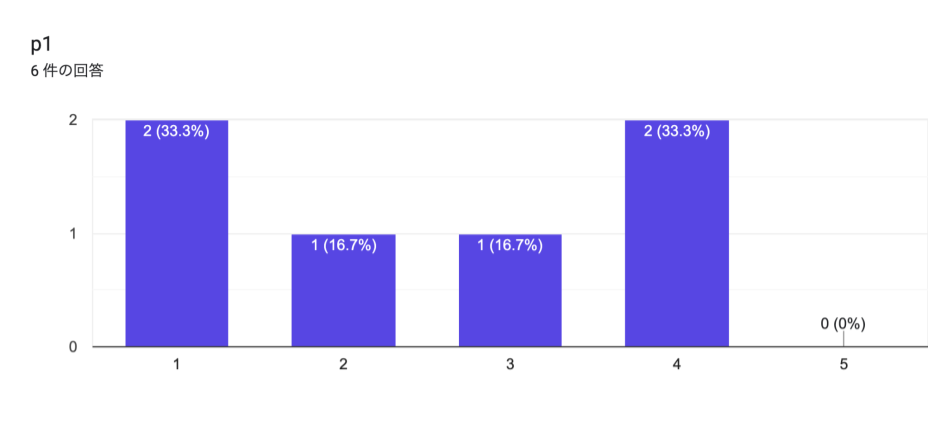
\includegraphics[width=0.75\linewidth]{figures/experiment/p1_1.png}
  \caption{P1（Default）の評価結果}
  \label{fig:p1_result}
\end{figure}

\paragraph{P2：Depth}

P2（Depth）は、端末の傾きに応じたパララックスを比較的強く設定したプリセットである。また、ちらつきを端末の動きと連動させることで、端末操作に応じた表示変化を強調している。P2に対する5段階評価の結果を図\ref{fig:p2_result}に示す。
\begin{figure}[H]
  \centering
  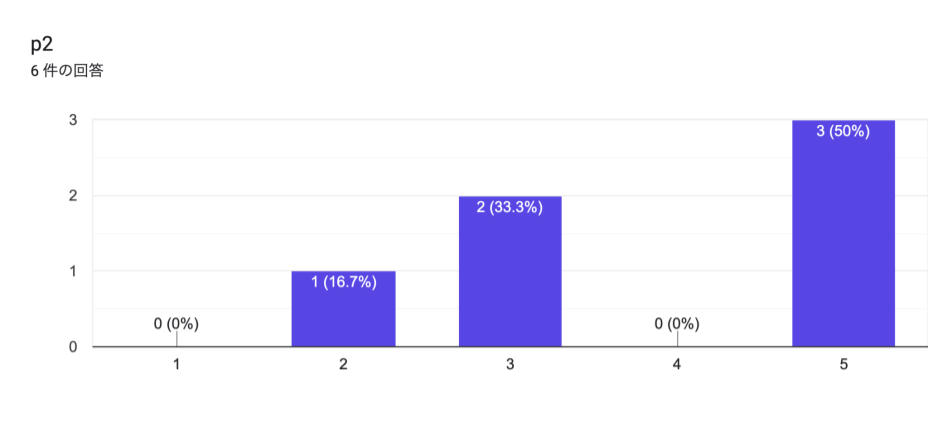
\includegraphics[width=0.75\linewidth]{figures/experiment/p2_1.png}
  \caption{P2（Depth）の評価結果}
  \label{fig:p2_result}
\end{figure}

\paragraph{P3：Vivid}

P3（Vivid）は、鮮やかな配色を用いるとともに、RGBずれおよびノイズを比較的大きく設定したプリセットである。色彩変化とグリッチの強度をともに強調した表現として構成した。P3に対する5段階評価の結果を図\ref{fig:p3_result}に示す。
\begin{figure}[H]
  \centering
  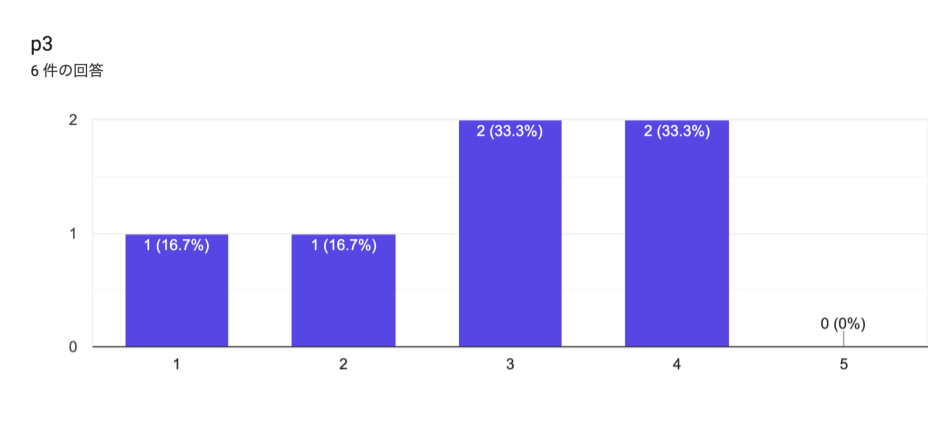
\includegraphics[width=0.75\linewidth]{figures/experiment/p3_1.png}
  \caption{P3（Vivid）の評価結果}
  \label{fig:p3_result}
\end{figure}

\paragraph{P4：Thin}

P4（Thin）は、帯状ノイズを細くし、ノイズサイズも比較的小さく設定したプリセットである。また、ちらつきを無効とすることで、他のプリセットと比較して細かく静かなグリッチ表現となるよう構成した。P4に対する5段階評価の結果を図\ref{fig:p4_result}に示す。
\begin{figure}[H]
  \centering
  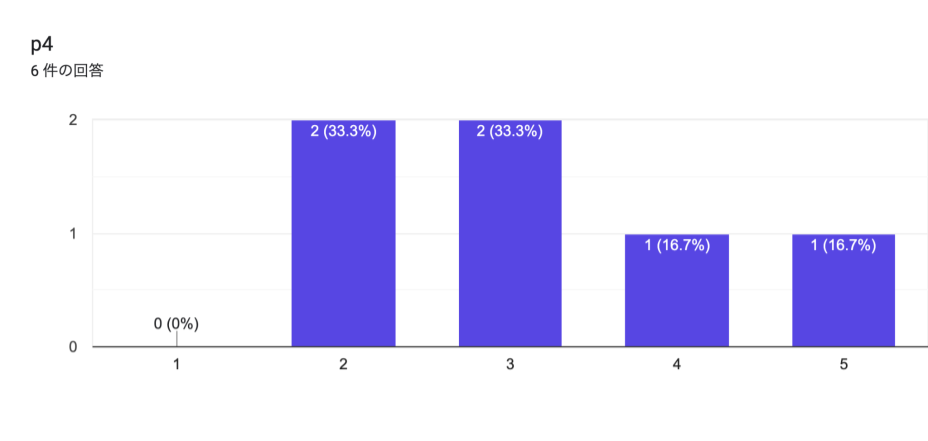
\includegraphics[width=0.75\linewidth]{figures/experiment/p4_1.png}
  \caption{P4（Thin）の評価結果}
  \label{fig:p4_result}
\end{figure}

\paragraph{P5：Corrupt}

P5（Corrupt）は、大きなノイズと強いちらつきを用い、画面の破損感を強調したプリセットである。また、鮮やかな配色を組み合わせることで、視覚的な変化量の大きい表現として構成した。P5に対する5段階評価の結果を図\ref{fig:p5_result}に示す。
\begin{figure}[H]
  \centering
  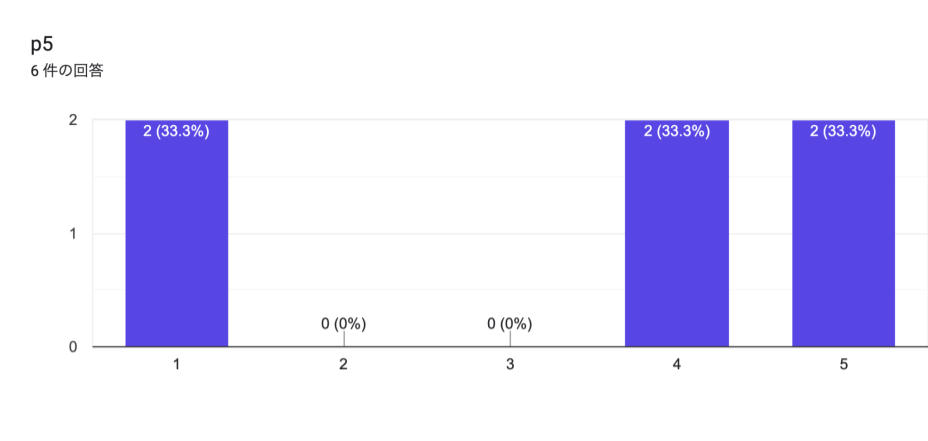
\includegraphics[width=0.75\linewidth]{figures/experiment/p5_1.png}
  \caption{P5（Corrupt）の評価結果}
  \label{fig:p5_result}
\end{figure}


\paragraph{P6：Drift}

P6（Drift）は、8種類のプリセットの中で最もパララックスを強く設定したものである。端末を傾けた際のレイヤ間の移動量の差を大きくすることで、グリッチ要素の移動と擬似的な奥行き感を強調した。P6に対する5段階評価の結果を図\ref{fig:p6_result}に示す。
\begin{figure}[H]
  \centering
  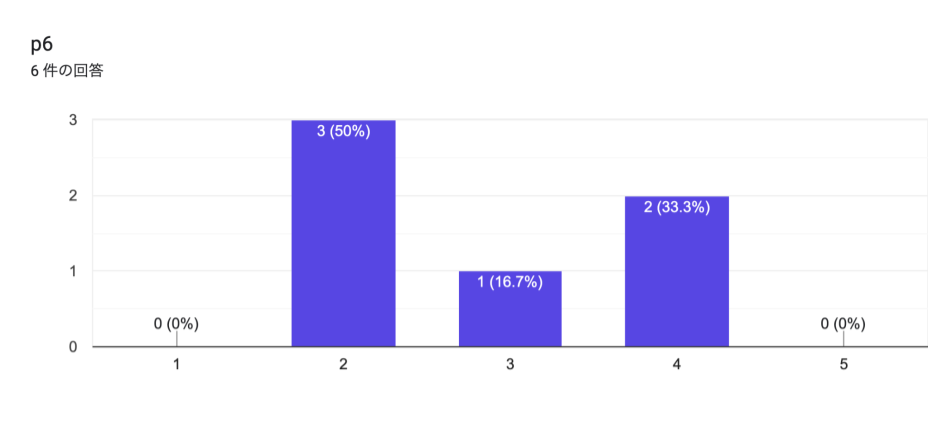
\includegraphics[width=0.75\linewidth]{figures/experiment/p6_1.png}
  \caption{P6（Drift）の評価結果}
  \label{fig:p6_result}
\end{figure}

\paragraph{P7：Quiet}

P7（Quiet）は、小さなノイズと控えめなRGBずれを用い、ちらつきを無効としたプリセットである。グリッチ表現の視覚的な刺激を比較的抑えた構成としている。P7に対する5段階評価の結果を図\ref{fig:p7_result}に示す。
\begin{figure}[H]
  \centering
  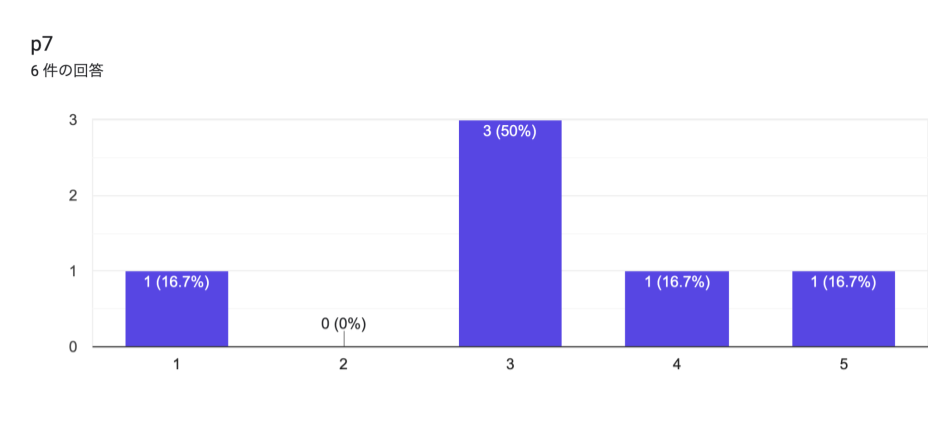
\includegraphics[width=0.75\linewidth]{figures/experiment/p7_1.png}
  \caption{P7（Quiet）の評価結果}
  \label{fig:p7_result}
\end{figure}

\paragraph{P8：Neon}

P8（Neon）は、RGBずれ、帯状ノイズの幅、色のばらつきを8種類の中で大きく設定したプリセットである。色成分の分離と広い帯状の変化を組み合わせ、色彩的なグリッチ表現を強調した。P8に対する5段階評価の結果を図\ref{fig:p8_result}に示す。
\begin{figure}[H]
  \centering
  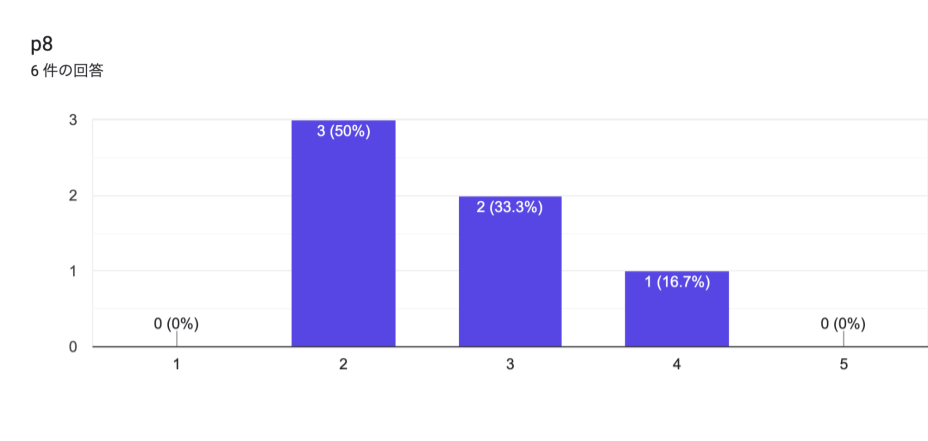
\includegraphics[width=0.75\linewidth]{figures/experiment/p8_1.png}
  \caption{P8（Neon）の評価結果}
  \label{fig:p8_result}
\end{figure}

\subsection{評価結果のまとめ}

8種類のライブ壁紙に対する評価を比較すると、特定のプリセットがすべての参加者から一様に支持される傾向は見られず、各壁紙に対する評価には参加者間でばらつきが確認された。特に、グリッチの強度、色彩、RGBずれ、視差効果などの異なる特徴を持つ壁紙に対して、参加者ごとの評価傾向は一様ではなかった。

この結果から、ライブ壁紙におけるグリッチ表現には単一の最適な設定を定めることが難しく、ユーザによって好まれる表現が異なる可能性が示唆された。本予備評価は、本研究において表現のパーソナライズへ着目する契機となった。そこで以降のシステムでは、あらかじめ定めたプリセットのみを提示するのではなく、ユーザ自身がグリッチの種類や強度、色彩等を調整できる構成へと設計方針を変更した。

\section{考察と今後の方針}

本評価では、当初、8種類のグリッチ表現を比較することで、多くの利用者から共通して高く評価される表現を明らかにすることを想定していた。

しかし、評価結果では、特定の一種類のみがすべての参加者から一貫して高く評価される傾向は確認できなかった。参加者によって高く評価する壁紙が異なり、同一のグリッチ表現に対する評価にも差がみられた。

この結果から、本研究で扱うグリッチ表現について、単一の表現を最適なものとして決定するだけでは、利用者ごとの選好の違いを十分に扱えない可能性があると考えた。そこで、予備評価以降は、一つの最適なグリッチ表現を探索する方向から、利用者が自身の選好に応じて異なる表現を選択できる構成を検討する方向へ研究方針を変更した。

ただし、本評価の参加者は6名と少なく、同一ゼミに所属する近い年齢層の学生に限定されている。また、評価項目も各壁紙に対する好ましさの5段階評価のみであり、参加者がどの視覚的要素を理由として評価したのかまでは明らかにできていない。

したがって、本評価の結果は一般的な利用者全体の選好を示すものではなく、今後の評価方法およびシステム設計を検討するための予備的な結果として位置付ける。
\chapter{システムおよび評価方法の改良}

\section{予備評価を踏まえた設計方針}

\section{グリッチ表現の改良}

\section{UIの改良}

\section{パーソナライズ機能}

\section{評価方法の再設計}

\chapter{本評価}

\section{評価目的}

\section{実験条件}

\section{評価方法}

\section{結果}

\section{分析}

\chapter{考察}

\section{グリッチ表現に対する選好}

\section{動的表現が壁紙利用に与える影響}

\section{個人差}

\section{パーソナライズの有効性}

\section{本研究の限界}

\chapter{結論}

\section{本研究のまとめ}

\section{今後の課題}


\printbibliography[heading=bibintoc,title={参考文献}]
% 謝辞が必要になったら、ここに \chapter*{謝辞} と本文を追加する。
\end{document}
